\documentclass[10pt, oneside]{amsdtx}

\usepackage{geometry}
\usepackage{graphicx}
\usepackage{amssymb}
\usepackage{amsthm}
\usepackage{amsmath}
\usepackage{xcolor}
\usepackage{tcolorbox}
\usepackage{pifont}
% \usepackage{mathpazo}
\usepackage{listings}
\usepackage{float}
\usepackage{booktabs}
\usepackage{enumitem}

\newcommand{\codetext}[1]{{\texttt{#1}}}

\definecolor{darkgreen}{rgb}{0.0, 0.5, 0.0}

\lstset{
  language = R,
  basicstyle=\ttfamily\small, % Monospaced font to match Palatino's elegance
  keywordstyle=\bfseries, % Bold blue for keywords
  commentstyle=\itshape\color{gray}, % Italic green for comments
  stringstyle=\color{darkgreen}, % Red for strings
  stepnumber=5, % Number every line
  breaklines=true, % Allow line breaking
  tabsize=2, % Tab width
}

\numberwithin{equation}{section}

\newcommand{\threedsquare}{\ding{113}}

\newtheoremstyle{theorem}% name
  {}%                                      Space above, empty = `usual value'
  {}%                                      Space below
  {\itshape}%                              Body font
  {}%                                      Indent amount 
  {\bfseries\color[HTML]{000575}}%         Head font
  { – }%                                   Punctuation after head
  { }%                                     Space after head: \newline = linebreak
  {\threedsquare \, \thmnote{#3}}%         Head spec
\theoremstyle{theorem}
\newtheorem{thm}{Theorem}[section]

\newtheoremstyle{definition}% name
  {}%                                      Space above, empty = `usual value'
  {}%                                      Space below
  {\itshape}%                              Body font
  {}%                                      Indent amount 
  {\bfseries\color[HTML]{650000}}%         Head font
  { – }%                                   Punctuation after head
  { }%                                     Space after head: \newline = linebreak
  {\threedsquare \, \thmnote{#3}}%         Head spec
\theoremstyle{definition}
\newtheorem{defn}{thm}[section]

\title{Machine Learning for Factor Investing}
\author{Albert Schrøder}


\begin{document}

\maketitle

\newpage

\chapter{Introduction}

\section{Notations and data}

\subsection{Notations}

\subsubsection{General notation}
Bold notations indicate vectors and matrices. We use capital letters for matrices and lower case letters for vectors. $\mathbf{v}'$ and $\mathbf{M}'$ denote the transpose. $\mathbf{M} = [m]_{i,j}$, where $i$ is the row index and $j$ is the column index.

Canonical matrices: $\mathbf{I}_{N}$ is the $(N \times N)$ identity matrix.

\subsubsection{Machine learning notation}
Two sets of notation. Machine learning notation in which the labels (also called output, dependent variables or predicted variables) $\mathbf{y} = y_{i}$ are approximated by functions of features $\mathbf{X}_{i}=(x_{i,1},\ldots,x_{i,K})$. Dimension of the feature matrix $\mathbf{X}$ is $I \times K$;  there are 
$I$ instances, records, or observations and each one of them has $K$ attributes, features, inputs, or predictors which will serve as independent variables. $\mathbf{x}_{i}$ is one instance (one row) of $\mathbf{X}$ and $\mathbf{x}_{k}$ is one feature (one column) vector of $\mathbf{X}$.

\subsubsection{Finance notation}
The second notation type pertains to finance and will directly relate to the first. We will often work with discrete returns $r_{t,n} = p_{t,n}/p_{t-1,n} - 1$. $t$ is the time index and $n$ is the asset index. The number of return dates is $T$, number of assets is $N$. The features or characteristics of assets will be denoted with $x_{t,n}^{(k)}$; the time-$t$ value of the $k^{th}$ attribute of firm/asset $n$. Stacked notation, $\mathbf{x}_{t,n}$, is the vector of characteristics of asset $n$ at time $t$. $\mathbf{r}_{t}$ is all returns at time $t$, and $\mathbf{r}_{n}$ is all returns of assets $n$. For the riskless asset we wil use $r_{t,f}$.

\subsubsection{Notation link}
The link between notation is: One \textit{instance} (or \textit{observation}) $i$ will consist of one couple $(t,n)$ of on e particular date and one particular firm (if data is rectangular with no missing field, $I = T \times N$). The label will usually be some performance measure of the firm computed over some future period, while the features will consist of the firm attributes at time 
$t$.

\subsubsection{Probabilistic notation}
The expectation operator is $\mathbb{E}[ \cdot ]$ and the conditional expectation $\mathbb{E}_{t}(\cdot)$, where the corresponding filtration $\mathcal{F}_{t}$ corresponds to all information available at time $t$; $\mathbb{E}_{t}[ \cdot ]  = \mathbb{E}[ \cdot | \mathcal{F}_{t}]$. 

$\mathbb{V}[ \cdot ]$ is the variance operator. Probabilities will be written $P$, but at times it will be $\mathbb{P}$. 

Probability density functions (pdfs) will be denoted with lowercase letters $(f)$ and cumulative distribution functions (cdfs) with uppercase letters $(F)$. Equality in distribution is $X \overset{d}{=} Y \iff F_{X}(z) = F_{Y}(z)$for all $z$ on the support of the variables. For a random process $X_{t}$ we say that it is \textit{stationary} if $X_{t}$ is constant trough time, i.e. $X_{t} \overset{d}{=} X_{s}$, where $\overset{d}{=}$ is equality in distribution.

Some asymptotic behaviors will be characterized with the usual Landau notation $o( \cdot )$ and $O( \cdot )$. $\varpropto$ refers to proportionality: $x \varpropto y$ means that $x$ is proportional to $y$. Derivatives use standard notation $\frac{\partial }{\partial x}$, and the compact symbol $\nabla$ is used when all derivatives are computed (gradient vector).

\subsubsection{Equations and functions}
In equations, the left-hand side and right-hand side can be written more compactly: l.h.s. and r.h.s., respectively.

Finally, we turn to functions. We list a few below:
\begin{itemize}
    \item $1_{\{ x \}}$: the indicator function of the condition $x$.
    \item $\phi( \cdot )$ and $\Phi( \cdot )$ are Gaussian pdf and cdf.
    \item $\operatorname{card}( \cdot ) = \#( \cdot )$ are two notations for the cardinal function which evaluates the number of elements in a given set.
    \item $\lfloor \cdot \rfloor$ is the integer part function.
    \item for a real number $x$, $[x]^{+}$ is the positive part of $x$, i.e., $\max(0,x)$.
    \item $\tanh( \cdot )$ is the hyperbolic tangent: $\tanh (x) = \frac{e^{ x }-e^{ -x }}{e^{ x }+e^{ -x }}$.
    \item $\operatorname{ReLu}( \cdot )$ is the rectified linear unit: $\operatorname{ReLu}( x ) = \max(0,x)$.
    \item $s( \cdot )$ is the softmax function: $s(\mathbf{x})_{i} = \frac{e^{ x_{i} }}{\sum _{j=1}^{J}e^{x_{j}}}$ where the subscript $i$ refers to the $i^{th}$ element of the vector.
\end{itemize}


\subsection{Dataset}
Throughout the book, and for the sake of reproducibility, we will illustrate the concepts we present with examples of implementation based on a single financial dataset available at \href{https://github.com/shokru/mlfactor.github.io/tree/master/material}{GitHub}. This dataset comprises information on 1,207 stocks listed in the US (possibly originating from Canada or Mexico). The time range starts in November 1998 and ends in March 2019. For each point in time, 93 characteristics describe the firms in the sample.

The sample is not perfectly rectangular: there are no missing points, but the number of firms and their attributes is not constant through time. This makes the computations in the backtest more tricky, but also more realistic.

There are four immediate labels in the dataset: \texttt{R1M\_Usd}, \texttt{R3M\_Usd}, \texttt{R6M\_Usd} and \texttt{R12M\_Usd}, which correspond to the 1-month, 3-month, 6-month and 12-month future/forward returns of the stocks. The returns are total returns, that is, they incorporate potential dividend payments over the considered periods. This is a better proxy of financial gain compared to price returns only.

In anticipation for future models, we keep the name of the predictors in memory. In addition, we also keep a much shorter list of predictors.
\begin{lstlisting}
features <- colnames(data_ml[3:95]) # Keep the feature's column names (hard-coded, beware!)
features_short <- c("Div_Yld", "Eps", "Mkt_Cap_12M_Usd", "Mom_11M_Usd",  "Ocf", "Pb", "Vol1Y_Usd")
\end{lstlisting}

The predictors have been uniformized, that is, for any given feature and time point, the distribution is uniform.

The original labels (future returns) are numerical and will be used for regression exercises, that is, when the objective is to predict a scalar real number. Sometimes, the exercises can be different and the purpose may be to forecast categories (also called classes), like “buy”, “hold” or “sell”. In order to be able to perform this type of classification analysis, we create additional labels that are categorical
\begin{lstlisting}
data_ml <- data_ml %>% 
group_by(date) %>%                                   # Group by date
mutate(R1M_Usd_C = R1M_Usd > median(R1M_Usd),        # Create the categorical labels
        R12M_Usd_C = R12M_Usd > median(R12M_Usd)) %>%
ungroup() %>%
mutate_if(is.logical, as.factor)
\end{lstlisting}

In machine learning, models are estimated on one portion of data (training set) and then tested on another portion of the data (testing set) to assess their quality. We split our sample accordingly.
\begin{lstlisting}
separation_date <- as.Date("2014-01-15")
training_sample <- filter(data_ml, date < separation_date)
testing_sample <- filter(data_ml, date >= separation_date)
\end{lstlisting}

\newpage

\section{Introduction}

\subsection{Context}
The rise of machine learning in factor investing is caused by three things: data availability, computational capacity, and economic groundings.

First, the \textbf{data}. Nowadays, classical providers, such as Bloomberg and Reuters have seen their playing field invaded by niche players and aggregation platforms. Hence, firm-specific attributes are easy and often cheap to compile. This means that the size of $\mathbf{X}$ in is now sufficiently large to be plugged into ML algorithms.

Second, \textbf{computational power}, both through hardware and software. Storage and processing speed are not technical hurdles anymore and models can even be run on the cloud thanks to services hosted by major actors (Amazon, Microsoft, IBM and Google) and by smaller players (Rackspace, Techila).

Finally, \textbf{economic framing}. Machine learning applications in finance were initially introduced by computer scientists and information system experts (e.g., Braun and Chandler (1987), White (1988)) and exploited shortly after by academics in financial economics (Bansal and Viswanathan (1993)), and hedge funds (see, e.g., Zuckerman (2019)). Nonlinear relationships then became more mainstream in asset pricing (Freeman and Tse (1992), Bansal, Hsieh, and Viswanathan (1993)). These contributions started to pave the way for the more brute-force approaches that have blossomed since the 2010 decade and which are mentioned throughout the book.

\textit{In the synthetic proposal of R. Arnott, Harvey, and Markowitz (2019), the first piece of advice is to rely on a model that makes sense economically}. This sentiment is believed to be be true in the following, and the only assumption is that future returns depend on firm characteristics. The relationship between these features and performance is largely unknown and probably time-varying. This is why ML can be useful: to detect some hidden patterns beyond the documented asset pricing anomalies. Moreover, dynamic training allows to adapt to changing market conditions.

\subsection{Portfolio construction: the workflow}
The following is focused on the prediction part. Allocating to assets requires to make bets and thus to presage and foresee which ones will do well. We mostly look at \textbf{supervised learning} to forecast returns in the cross-section. The baseline equation in supervised learning
\begin{equation}
    \mathbf{y} = f(\mathbf{X}) + \epsilon 
\end{equation}
which in financial terms is
\begin{equation}
    \mathbf{r}_{t+1,n} = f(\mathbf{x}_{t,n}) + \epsilon_{t+1,n}
\end{equation}
where $f(\mathbf{x}_{t,n})$ is the expected return for time $t+1$ computed at time $t$, i.e., $\mathbb{E}_{t}[r_{t+1},n]$. The model is common to all assets share ($f$ is not indexed by $n$), similarity with panel approaches.

Building accurate predictions requires to pay attention to all terms in the above equation. Chronologically, the first step is to gather data and to process it. The only consensus is the on the $\mathbf{x}$ side the features should include classical predictors reported in the literature: market capitalization, accounting ratios, risk measures, momentum proxies, etc. For the dependent variable, many researchers and practitioners work with monthly returns, but other maturities may perform better out-of-sample.

It is tempting to think that the most important part is the choice of $f$, but its likely the choice and engineering of inputs (the variables) is just as important. Finally, the errors $\epsilon_{t+1,n}$ are often overlooked. 

\subsection{Machine learning is no magic wand}
By definition, the curse of predictions is that they rely on past data to infer patterns about subsequent fluctuations. The more or less explicit hope of any forecaster is that the past will turn out to be a good approximation of the future. Needless to say, this is a pious wish; in general, predictions fare badly.

To illustrate this sad truth, the baseline algorithms that we detail in Chapters 5 to 7 yield at best mediocre results. This is done on purpose. This forces the reader to understand that blindly feeding data and parameters to a coded function will seldom suffice to reach satisfactory out-of-sample accuracy.

Below, are some key points: 
\begin{itemize}
    \item The first point is that causality is key. If  one is able to identify $\mathbf{X} \mapsto y$, where $y$ are expected returns, then the problem is solved. Unfortunately, causality is incredibly hard to uncover.
    \item Thus, researchers have most of the time to make do with simple correlation patterns, which are far less informative and robust.
    \item Relatedly, financial datasets are extremely noisy. It is a daunting task to extract signals out of them. No-arbitrage reasonings imply that if a simple pattern yielded durable profits, it would mechanically and rapidly vanish.
    \item The no-free lunch theorem imposes that the analyst formulates views on the model. This is why economic or econometric framing is key. The assumptions and choices that are made regarding both the dependent variables and the explanatory features are decisive. As a corollary, data is key. The inputs given to the models are probably much more important than the choice of the model itself.
    \item To maximize out-of-sample efficiency, the right question is probably to paraphrase Jeff Bezos: what's not going to change? Persistent series are more likely to unveil enduring patterns.
\end{itemize}



\newpage

\section{Factor investing and asset pricing anomalies}

Asset pricing anomalies are the foundations of factor investing. In this chapter our aim is twofold:
\begin{itemize}
    \item present simple ideas and concepts: basic factor models and common empirical facts
    \item provide a last of articles that go deeper on the topic.
\end{itemize}

This chapter is to create a broad overview of topics related to factor investing. For academically oriented studies look at \textit{Journal of Finance}, the \textit{Review of Financial Studies} and the \textit{Journal of Financial Economics}. For practitioner-oriented papers look at \textit{Journal of Portfolio Management} and the \textit{Financial Analysts Journal}.

\subsection{Introduction}
The core aim of factor models is to understand the \textbf{drivers of asset prices}.The rationale behind factor investing is that the \textit{financial performance of firms depends on factors, whether they be latent and unobservable, or related to intrinsic characteristics}. Cochrane (2011) frames the first essential question: \textit{which characteristics really provide independent information about average returns?}.

Linear factor models can be viewed as special cases of the arbitrage pricing theory (APT) of Ross (1976), which assumes that the return of an asset $n$ can be modelled as a linear combination of underlying factors $\boldsymbol{f_{k}}$:
\begin{equation}
    r_{t,n} = \alpha_{n} + \sum_{k=1}^{K} \beta_{n,k} \boldsymbol{f}_{t,k} + \epsilon_{t,n}, \label{eq:3}
\end{equation}
where the usual constraints on linear models hold: $\mathbb{E}[\epsilon _{t,n}] = 0$, $\operatorname{cov}(\epsilon _{t,n}, \epsilon_{t,m}) = 0$ for $n \neq m$ and $\operatorname{cov}(\mathbf{f}_{n}, \mathbf{\epsilon}_{n}) = 0$. If such factors do not exist then they are in contradiction with CAPM, which is the corner stone model of asset pricing. According to CAPM the only driver of returns is the market portfolio. This explains why factors are also called '\textit{anomalies}'. Pesaran and Smith (2021), the authors define the strength of factors using the sum of squared $\beta _{n,k}$ (across firms).

The regression \eqref{eq:3} can be evaluated once (unconditionally) or sequentially over different time frames. In the latter case, the parameters (coefficient estimates) change and the models are thus called \textit{conditional}. Conditional models are more flexible because they acknowledge that the drivers of asset prices may not be constant.

\subsection{Detecting anomalies}

\subsubsection{Challenges}
A crucial step is to be able to identify an anomaly and the complexity of this task should not be underestimated. Many findings are not reproducible. Nevertheless, as is demonstrated by A. Y. Chen (2019), $p$-hacking alone cannot account for all the anomalies documented in the literature. One way to reduce the risk of spurious detection is to increase the hurdles, or to resort to multiple testing. Nevertheless, the large sample sizes used in finance may mechanically lead to very low $p$-values.

The destruction of factor premia may be due to herding and could be accelerated by the democratization of so-called smart-beta products (ETFs notably) that allow investors to directly invest in particular styles. The book mentions a lot of different challenges, that are not shown in these notes. 

\subsubsection{Simple portfolio sort}
This is the most common procedure and it is used by Farma and French. The idea is simple. On one date, 
\begin{enumerate}
    \item rank firms according to a particular criterion (e.g, size, book-to-market ratio);
    \item form $J \geq 2$ portfolios (i.e. homogeneous groups) consisting of the same number of stocks according to the ranking (usually, $J=2$, $J=3$, $J=5$, or $J=10$ portfolios are built based on the median, terciles, quintiles or deciles of the criterion);
    \item the weight of stocks inside the portfolio is either uniform or proportional to market capitalization;
    \item at a future date (usually one month), report the returns of the portfolios. Then iterate the procedure until the chronological end of the sample is reached. 
\end{enumerate}

The outcome is a time series of portfolio returns $r_{t}^{j}$ for each grouping $j$. An anomaly is identified if the $t$-test between the first ($j=1$) and the last group ($j=J$) unveils a significant difference in average returns.  A strong limitation of this approach is that the sorting criterion could have a non-monotonic impact on returns and a test based on the two extreme portfolios would not detect it. Another concern is that these sorted portfolios may capture not only the priced risk associated to the characteristic, but also some unpriced risk.

Instead of focusing on only one criterion, it is possible to group asset according to more characteristics. The original paper (\textit{Fama and French (1992)}) also combines market capitalization with book-to-market ratios. Each characteristic is divided into 10 buckets, which makes 100 portfolios in total. There is no upper bound on the amount of features that can be included.

Olivier Ledoit, Wolf, and Zhao (2020) take into account the covariance structure of asset returns and to Cattaneo et al. (2020) for a theoretical study on the statistical properties of the sorting procedure (\textit{including theoretical links with regression-based approaches}). Notably, the latter paper discusses the optimal number of portfolios and suggests that it is probably larger than the usual 10 often used in the literature.

In the code below size portfolios are computes (equally weighted: above versus below the median capitalization). According to the size anomaly\footnote{Size anomaly: smaller companies (measured by market capitalization) tend to generate higher average returns compared to large companies over the long term.}, firms with below median market cap should earn higher returns on average. This is verified when the orange bar in the plot is above the blue one:

\begin{lstlisting}
data_ml |> 
    group_by(date) |> 
    mutate(large = Mkt_Cap_12M_Usd > median(Mkt_Cap_12M_Usd)) |> 
    ungroup() |> 
    mutate(year = lubridate::year(date)) |> 
    group_by(year, large) |> 
    summarise(avg_return = mean(R1M_Usd)) |> 
    ggplot(aes(x = year, y = avg_return, fill = large)) + 
    geom_col(position = "dodge") + 
    scale_fill_manual(values = c("#F8766D", "#619CFF"), labels = c("Small", "Large"), name = "") + 
    ylab("Average returns") +
    theme_minimal()
\end{lstlisting}

This gives the following histogram, which confirms the size anomaly (i.e., smaller companies tend to yield higher returns over time)
\begin{figure}[H]
    \caption{Size anomaly plot}
    \centering
    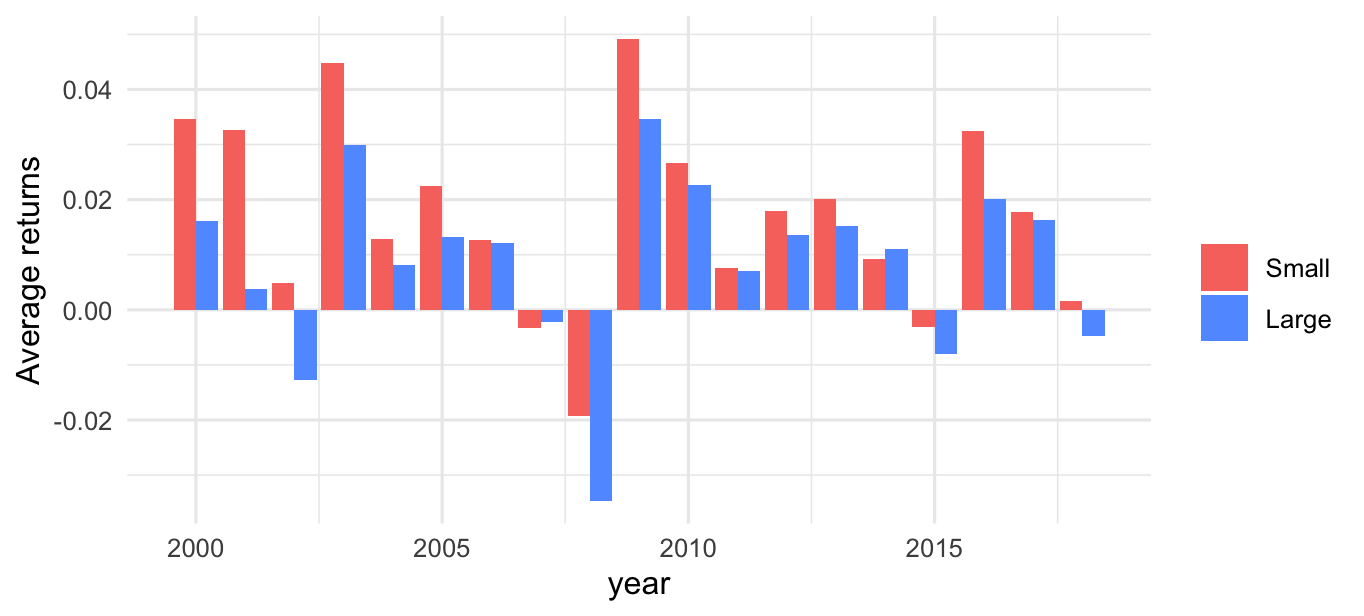
\includegraphics[width=0.75\textwidth]{part_1/images/size_anomaly.png}
\end{figure}


\subsubsection{Factors}
Factors are constructed like done above. Portfolios are based on one characteristic and the factor is a long-short ensemble of one extreme portfolio minus the opposite extreme (\textit{e.g., small minus large for the size factor or high book-to-market ratio minus large book-to-market-ratio for the value factor}). Sometimes, subtleties include forming bivariate sorts and aggregating several portfolios together. 

The most common factors are listed below, along with a few references. Look at the books listed at the beginning of the chapter for a more exhaustive treatment of factor idiosyncrasies.
\begin{itemize}
    \item Size (\textbf{SMB}): small firms minus large firms.
    \item Value (\textbf{HML}): high minus low: undervalues minus 'growth' firms.
    \item Momentum (\textbf{WML}): winners minus losers.
    \item Profitability (\textbf{RMW}): robust minus weak profits.
    \item Investment (\textbf{CMA}): conservative minus aggressive.
    \item Low 'risk' (\textbf{BAB}): betting against beta.
\end{itemize}

With the notable exception of the low risk premium, the most mainstream anomalies are kept and updated in the data library of Kenneth French (\href{https://mba.tuck.dartmouth.edu/pages/faculty/ken.french/data_library.html}{Dartmouth data library}). The computation of these factors follows a set of rules. Another source for data is the AQR repo: \href{https://www.aqr.com/Insights/Datasets}{AQR repository}.

These notes use a proxy for the value anomaly (\textit{I use not the book-to-market ratio, but price-to-book ratio}).

Below data from Ken French's data library is imported.
\begin{lstlisting}
min_date <- "1963-07-31"                  # Start date
max_date <- "2020-03-28"                  # Stop date

# Get KF data file of factors
temp <- tempfile()
KF_website <- "http://mba.tuck.dartmouth.edu/pages/faculty/ken.french/"
KF_file <- "ftp/F-F_Research_Data_5_Factors_2x3_CSV.zip"
link <- paste0(KF_website, KF_file)       # Link to file
download.file(link, temp, quiet = TRUE)   # Download file

# Clean up dataframe 
FF_factors <- read_csv(unz(temp, "F-F_Research_Data_5_Factors_2x3.csv"), skip = 3) |> 
  rename(date = '...1', MKT_RF = 'Mkt-RF') |> 
  mutate_at(vars(-date), as.numeric) |> 
  mutate(date = ymd(parse_date_time(date, "%Y%m"))) |> 
  mutate(date = rollback(date + months(1)))

# Scale returns
FF_factors <- FF_factors |> 
  mutate(
    MKT_RF = MKT_RF/100,
    SMB = SMB / 100,
    HML = HML / 100,
    RMW = RMW / 100,
    CMA = CMA / 100,
    RF = RF/100) |> 
  filter(date >= min_date, date <= max_date)
\end{lstlisting}

The six factors used by Farma and French can be seem below as they have been imported form Ken French's website:
\begin{table}[H]
    \centering
    \begin{tabular}[t]{lrrrrrr}
    \toprule
    date & MKT\_RF & SMB & HML & RMW & CMA & RF\\
    \midrule
    1963-07-31 & -0.0039 & -0.0041 & -0.0097 & 0.0068 & -0.0118 & 0.0027\\
    1963-08-31 & 0.0507 & -0.0080 & 0.0180 & 0.0036 & -0.0035 & 0.0025\\
    1963-09-30 & -0.0157 & -0.0052 & 0.0013 & -0.0071 & 0.0029 & 0.0027\\
    1963-10-31 & 0.0253 & -0.0139 & -0.0010 & 0.0280 & -0.0201 & 0.0029\\
    1963-11-30 & -0.0085 & -0.0088 & 0.0175 & -0.0051 & 0.0224 & 0.0027\\
    1963-12-31 & 0.0183 & -0.0210 & -0.0002 & 0.0003 & -0.0007 & 0.0029\\
    \bottomrule
    \end{tabular}
\end{table}

While these factors (i.e., long-short portfolios) exhibit time-varying risk premia and are magnified by corporate news and announcements, it is well-documented (and accepted) that they deliver positive returns over long horizons. it is well-documented (and accepted) that they deliver positive returns over long horizons and estimation methods can be improved.

Below we plot the average monthly return aggregated over each calendar year for five common factors. The risk free rate (which is not a factor per se) is the most stable, while the market factor (aggregate market returns minus the risk-free rate) is the most volatile. This makes sense because it is the only long equity factor among the five series.
\begin{lstlisting}
FF_factors |> 
  mutate(date = year(date)) |> 
  gather(key = factor, value = value, -date) |> 
  group_by(date, factor) |> 
  summarise(value = mean(value)) |> 
  ggplot(aes(x = date, y = value, color = factor)) + 
  geom_line() + 
  coord_fixed(200) + 
  theme_minimal()
\end{lstlisting}
\begin{figure}[H]
    \centering
    \caption{Average returns of common anomalies}
    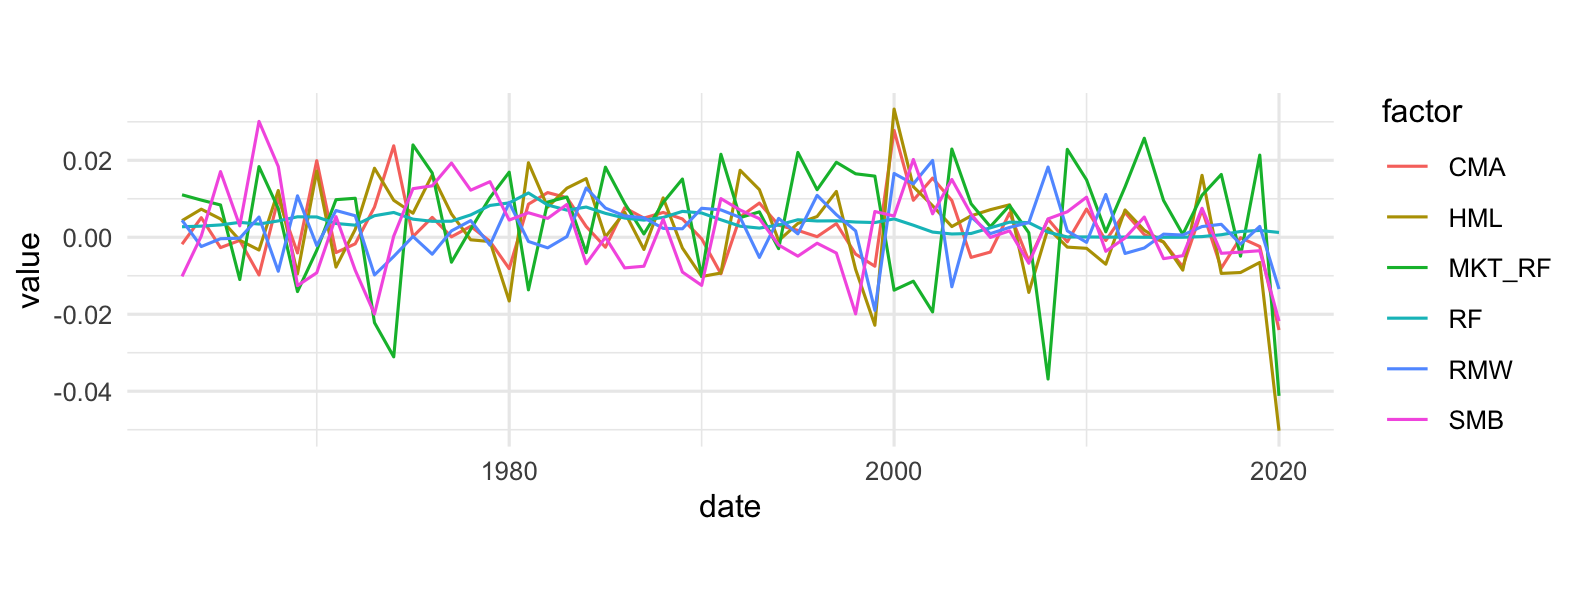
\includegraphics[width=0.85\textwidth]{part_1/images/factor_vals.png}
\end{figure}

As is shown by Linnainmaa and Roberts (2018) and Hou, Xue, and Zhang (2020), many proclaimed factors are in fact very much data-dependent and often fail to deliver sustained profitability when the investment universe is altered or when the definition of variable changes. Campbell Harvey and his co-authors, in a series of papers, tried to synthesize the research on factors in C. R. Harvey, Liu, and Zhu (2016), C. Harvey and Liu (2019) and C. R. Harvey and Liu (2019). His work underlines the need to set high bars for an anomaly to be called a \textit{true} factor. Increasing thresholds for $p$-values is only a partial answer, as it is always possible to resort to data snooping in order to find an optimized strategy that will fail out-of-sample but that will deliver a $t$-statistic larger than three (or even four). C. R. Harvey (2017) recommends to resort to a Bayesian approach which blends data-based significance with a prior into a so-called Bayesianized $p$-value.

Bryzgalova, Huang, and Julliard (2019) propose a tractable Bayesian estimation of large-dimensional factor models and evaluate all possible combinations of more than 50 factors, yielding an incredibly large number of coefficients. This combined with a Bayesianized Fama and MacBeth (1973) procedure allows to distinguish between pervasive and superfluous factors. Chordia, Goyal, and Saretto (2020) use simulations of 2 million trading strategies to estimate the rate of \textit{false discoveries}, that is, when a spurious factor is detected (type I error). They also advise to use thresholds for t-statistics that are well above three. In a similar vein, C. R. Harvey and Liu (2020) also underline that sometimes true anomalies may be missed because of a one time $t$-statistic that is too low (type II error).

The propensity of journals to publish positive results has led researchers to estimate the difference between reported returns and true returns. A. Y. Chen and Zimmermann (2020) call this difference the publication bias and estimate it as roughly 12\%. That is, if a published average return is 8\%, the actual value may in fact be closer to $(1-12\%)*8\%=7\%$. Qualitatively, this estimation of 12\% is smaller than the out-of-sample reduction in returns found in McLean and Pontiff (2016).

\subsubsection{Predective regressions, sorts, and $p$-value issues}
For simplicity, we assume a simple form:
\begin{equation}
    \mathbf{r} = a + b \mathbf{x} + \mathbf{e}
\end{equation}
where vector $\mathbf{r}$ stacks all returns of stocks and $\mathbf{x}$ is a lagged variable (\textit{regression is therefore predictive}). If $\hat{b}$ is significant given a specific threshold, then it can be tempting to conclude that $\mathbf{x}$ is a good predictor of returns. Hence, long-short portfolios related to extreme values of $\mathbf{x}$ are expected to to generate profits. This is not true, since $\hat{b}$ gives information on the past ability of $\mathbf{x}$ to forecast results. What is about to happen may be a different story.


Statistical tests are also used for portfolio sorts. Assume two extreme portfolios are expected to yield very different average returns. The portfolio returns are written as $r_{t}^{+}$ and $r_{t}^{-}$. The simplest test for the mean is $t = \sqrt{T}\frac{m_{r_{+}} - m_{r_{-}}}{\sigma_{r_{+} - r_{-}}}$, where $T$ is the number of points and $m_{r_{+}}$ denotes the means of returns and $\sigma _{r_{+} - r_{-}}$ is the standard deviation of the difference between the two series (\textit{i.e., volatility of the long-short portfolio}). The statistic can be viewed as a scaled Sharpe-ratio and can in turn be used to compute the $p$-values to assess the robustness of an anomaly. Many factors discovered by researchers fail to survive in out-of-sample tests.


One reason why people are overly optimistic about anomalies they detect is the widespread reverse interpretation of the $p$-value. Often, it is thought of as the probability of one hypothesis (\textit{e.g., my anomaly exists}) given the data. In fact, it's the opposite; it's the likelihood of your data sample, knowing that the anomaly holds.
\begin{align*}
    p & = P[D|H] \\
    \text{target prob} & = P[H|D]= \frac{P[D|H]}{P[D]} \cdot P[H]
\end{align*}
where $H$ standard for the hypothesis and $D$ for data. The equality in the second row is an application of Bayes' identity: the interesting probability is a transform of the $p$-value.

C. R. Harvey (2017) introduces Bayesianized $p$-values (Bpv)
\begin{equation*}
    \text{Bpv} = e^{ -\frac{t^{2}}{2} } \cdot \frac{\text{prior}}{1 + e^{ -\frac{t^{2}}{2} } \cdot \text{prior}}
\end{equation*}
where $t$ is the $t$-statistic from the regression (\textit{i.e., the one that defines the $p$-value}) and prior is the analyst's estimation of the odds that the hypothesis (anomaly) is true. The odds are coded as $p/(1-p)$. Thus, if the $t$-statistic is equal to 2 and the prior odds are equal to 6, then the Bpv is $e^{ -2 } \cdot 6 \cdot (1 + e^{ -2 } \cdot 6)^{-1} \approx 0.448$ and there is a $44.8\%$ chance the null is true. 

\subsubsection{Fama-McBeth regresssions}
Another detection method was proposed by Fama and MacBeth; two-stage regression analysis of risk prima. First step is a simple estimation of the relationship \eqref{eq:3}: the regressions are run on a stock-by-stock basis over corresponding time series. The resulting estimates $\hat{\beta}_{i,k}$ are plugged into a second series of regressions: 
\begin{equation*}
    r_{t,n} = \gamma _{t,0} + \sum _{k=1}^{K} \gamma _{t,k} \hat{\beta}_{n,k} + \varepsilon_{t,n}
\end{equation*}
which are run date-by-date on the cross-section of assets. Theoretically, the betas are known and the regression is run on $\beta _{n,k}$ instead of the estimated values. The $\hat{\gamma}_{t,k}$ estimate the premia of factor $k$ at time $t$. Under suitable distributional assumptions on $\varepsilon_{t,n}$, statistical test can be performed to determine whether these permia are significant or not. The statistical test most often used on the time-aggregated (average) premia $\hat{\gamma }_k = \frac{1}{T} \sum _{t=1}^{T} \hat{\gamma }_{t,k}$:
\begin{equation*}
    t_{k} = \frac{\hat{\gamma}_{k}}{\hat{\sigma}_{k}/\sqrt{T}} 
\end{equation*}
is often used in pure Gaussian contexts to assess whether or not the factor is significant ($\hat{\sigma }_k$ is the standard deviation of $\hat{\gamma}_{t,k}$).

Biases and losses in accuracy can be included by standard OLS estimations. Moreover, as the $\hat{\beta}_{i,k}$ in the second-pass regression are estimates, a second level of error can arise (called errors in variables). 

Below the Fama and MacBeth regressions are performed on our sample. We start by the first pass: individual estimation of betas. We build a dedicated function below and use some functional programming to automate the process. We stick to the original implementation of the estimation and perform synchronous regressions
\begin{lstlisting}
# Number of factors
nb_factors <- 5

# Create a dataframe with factors and all stock returns for a given date on each row
data_FM <- left_join(data_ml |> 
            dplyr::select(date, stock_id, R1M_Usd) |> 
            filter(stock_id %in% stock_ids_short), 
          FF_factors, 
          by = "date") |> 
  group_by(stock_id) |> 
  mutate(R1M_Usd = lag(R1M_Usd)) |> 
  ungroup() |> 
  na.omit() |> 
  pivot_wider(names_from = "stock_id", values_from = "R1M_Usd")

# Fit linear models of factors and returns over time for each stock 
models <- lapply(
  paste0("`", stock_ids_short, "`", " ~ MKT_RF + SMB + HML + RMW + CMA"), 
  function(f){ lm(as.formula(f), data = data_FM, na.action = "na.exclude") |> 
      summary() %>%
      "$"(coef) |> 
      data.frame() |> 
      dplyr::select(Estimate)}) 

# Format table of betas nicely
betas <- matrix(unlist(models), ncol = nb_factors + 1, byrow = TRUE) |> 
  data.frame(row.names = stock_ids_short)
colnames(betas) <- c("Constant", "MKT_RF", "SMB", "HML", "RMW", "CMA")
\end{lstlisting}

In the table below is a sample of the estimated betas for the first 6 stocks.
\begin{table}[H]
    \centering
    \begin{tabular}[t]{lrrrrrr}
    \toprule
      & Constant & MKT\_RF & SMB & HML & RMW & CMA\\
    \midrule
    1 & 0.0080073 & 1.4185896 & 0.5220226 & 0.6178794 & 0.9749334 & -0.3612393\\
    3 & -0.0022122 & 0.8115331 & 1.1048548 & 0.8853894 & 0.2972274 & -0.5544541\\
    4 & 0.0045092 & 0.3628417 & 0.3058171 & -0.0482520 & 0.5957859 & 0.1940631\\
    7 & 0.0053913 & 0.4310613 & 0.6745676 & 0.2316349 & 0.3212058 & 0.1723559\\
    9 & 0.0037773 & 0.8386114 & 0.6776150 & 1.0568940 & 0.0790805 & 0.0626698\\
    11 & -0.0011353 & 0.9842782 & 0.1179911 & 0.4887056 & -0.1288554 & 0.0112944\\
    \bottomrule
    \end{tabular}
\end{table}

Below we prepare the estimated betas for the second pass of regressions, where we bind the estimated factors for each stock to the stock returns of the same stock. 
\begin{lstlisting}
loadings <- betas |> 
  dplyr::select(-Constant) |> 
  data.frame()

ret <- returns |> 
  dplyr::select(-date) |> 
  data.frame(row.names = returns$date) |> 
  t()

FM_data <- cbind(loadings, ret)
\end{lstlisting}

We observe that the values of the first column (market betas) revolve around one, which is what we would expect. The second pass is done below, where try to estimate the effect of each factor on return of all stocks for a given date. We therefore get the factor prima for each day, which is how big the prima of each factor was every day.
\begin{lstlisting}
models <- lapply(
  paste("`", returns$date, "`", ' ~  MKT_RF + SMB + HML + RMW + CMA', sep = ""),
  function(f){ lm(as.formula(f), data = FM_data) |> 
      summary() %>%
      "$"(coef) |> 
      data.frame() |> 
      dplyr::select(Estimate)})

gammas <- matrix(unlist(models), ncol = nb_factors + 1, byrow = TRUE) |> 
  data.frame(row.names = returns$date)
colnames(gammas) <- c("Constant", "MKT_RF", "SMB", "HML", "RMW", "CMA") 

gammas[2:nrow(gammas),] |> 
  dplyr::select(MKT_RF, SMB, HML) %>% 
  bind_cols(date = data_FM$date) %>%
  gather(key = factor, value = gamma, -date) %>% 
  ggplot(aes(x = date, y = gamma, color = factor)) +
  geom_line() +
  facet_grid(factor ~.) + 
  theme_minimal()
\end{lstlisting}

Below is a plot showing the volatility of each market prima for factors over time. We observe that they are very volatile. 
\begin{figure}[H]
    \centering
    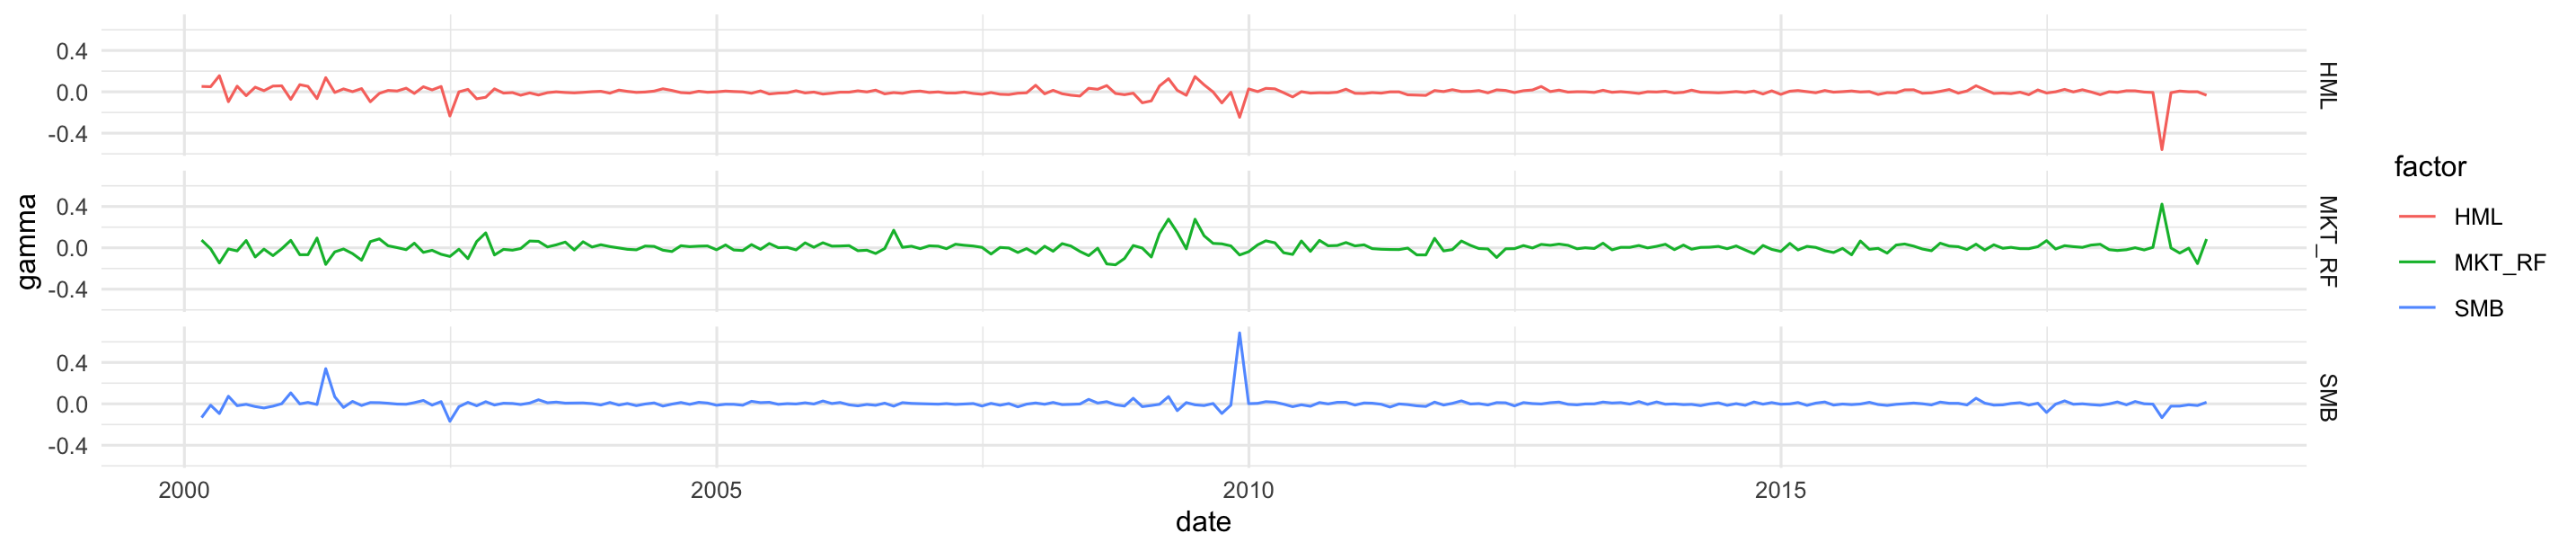
\includegraphics[width=0.95\textwidth]{part_1/images/factor_prima_markets.png}
\end{figure}

The two spikes at the end of the sample signal potential colinearity issues; two factors seem to compensate in an unclear aggregate effect. This underlines the usefulness of penalized estimates (discussed in later sections).

\subsubsection{Factor competition}
The core purpose of factors is to explain the cross-section of stock returns. For theoretical and practical reasons, it is preferable if redundancies within factors are avoided. Indeed, redundancies imply collinearity which is known to perturb estimates. In addition, when asset managers decompose the performance of their returns into factors, overlaps (high absolute correlations) between factors yield exposures that are less interpretable; positive and negative exposures compensate each other spuriously.

A simple protocol to sort out redundant factors is to run regressions of each factor against all others:
\begin{equation}
    f_{t,k} = a_{k} + \sum_{j \neq k} \delta_{k,j}f_{t,j} + \epsilon_{t,k} \label{eq:5}
\end{equation}
The metric of interest is the statistic associated with the estimation of $a_{k}$. If $a_{k}$ is significantly different from zero, then the cross-section of (other) factors fails to explain exhaustively the average return of factor. Otherwise, the return of the factor can be captured by exposures to the other factors and is thus redundant. In the regression above we try to estimate a factor for with all other factors. If we find that we need an additional terms to explain factor $k$ then they remaining factors fail to explain that factor $k$, i.e., that $k$ is not redundant; otherwise, we remaining factors $j \neq k$ can explain factor $k$ and thus imply redundancy.

One mainstream application of this technique was performed in Fama and French (2015), in which the authors show that the HML factor is redundant when taking into account four other factors (Market, SMB, RMW and CMA). This is shown below. 

We can run the regressions that determine the redundancy of factors via the procedure defined in \eqref{eq:5}.
\begin{lstlisting}
# All factors
factors <- c("MKT_RF", "SMB", "HML", "RMW", "CMA")

models <- lapply(
  paste(factors, ' ~ MKT_RF + SMB + HML + RMW + CMA - ', factors), 
  function(f){lm(as.formula(f), data = FF_factors) %>% 
      summary() %>% 
      "$"(coef) %>% 
      data.frame() %>% 
      filter(rownames(.) == "(Intercept)") %>% 
      dplyr::select(Estimate, `Pr...t..`)
    })

alphas <- matrix(unlist(models), ncol = 2, byrow = TRUE) %>% 
  data.frame(row.names = factors)
colnames(alphas) <- c("Estimate", "Signifcance")
alphas
\end{lstlisting}

This gives the following table of $\alpha$'s, where we can see that the factor HML is redundant when the four other factors are present in the pricing model. These results are close to those obtained in the study by Fama.
\begin{table}[H]
    \centering
    \begin{tabular}{lrr}
    \toprule
      & Estimate & Signifcance\\
    \midrule
    MKT\_RF & 0.0077969 & 0.0000004\\
    SMB & 0.0027418 & 0.0128758\\
    HML & -0.0005571 & 0.4884991\\
    RMW & 0.0038725 & 0.0000009\\
    CMA & 0.0023971 & 0.0000058\\
    \bottomrule
    \end{tabular}
\end{table}

Researchers also look at which factors maximize the likelihood of the observed data. Some papers seek to quantify to which extent the 3 factor model outperforms the 5 factor model.

\subsection{Hot topics: momentum, timing and ESG}

\subsubsection{Factor momentum}
A recent body of literature unveils a time series momentum property of factor returns. T. Gupta and Kelly (2019) report that autocorrelation patterns within these returns is statistically significant. Additional work points to the fact the industry momentum can be explained by factor momentum. In the extremes researches propose that the momentum factor is an aggregate of the autocorrelation found in all other factors\footnote{The strength of factor momentum has been scrutinized; the authors find that it is only robust for a small number of factors}.

H. Yang seeks to understand the source of factor momentum and decomposes stock factor momentum portfolios into two components: factor timing portfolio and a static portfolio. The former seeks to profit from the serial correlation of factor returns, whilst the latter tries to harness factor prima. The static portfolio explains a larger portion of factor momentum returns. H. Yang presents an estimator to gauge factor momentum predictability.

Given data obtained by Ken French, we compute the autocorrelation function of factors
\begin{equation*}
    \operatorname{ACF}_{k}(\mathbf{x}_{t}) = \mathbb{E}[(\mathbf{x}_{t} - \bar{\mathbf{x}})(\mathbf{x}_{t+k} - \bar{\mathbf{x}})]
\end{equation*}

\begin{lstlisting}
acf_SMB <- ggAcf(FF_factors$SMB, lag.max = 10) + labs(title = "") + theme_minimal()  # ACF SMB
acf_HML <- ggAcf(FF_factors$HML, lag.max = 10) + labs(title = "") + theme_minimal()  # ACF HML
acf_RMW <- ggAcf(FF_factors$RMW, lag.max = 10) + labs(title = "") + theme_minimal()  # ACF RMW
acf_CMA <- ggAcf(FF_factors$CMA, lag.max = 10) + labs(title = "") + theme_minimal()  # ACF CMA
plot_grid(acf_SMB, acf_HML, acf_RMW, acf_CMA,  # Plot
          labels = c('SMB', 'HML', 'RMW', 'CMA'))
\end{lstlisting}
which gives the following plots, where we observe that only the size factor is not significantly correlated at the first order.
\begin{figure}[H]
    \centering
    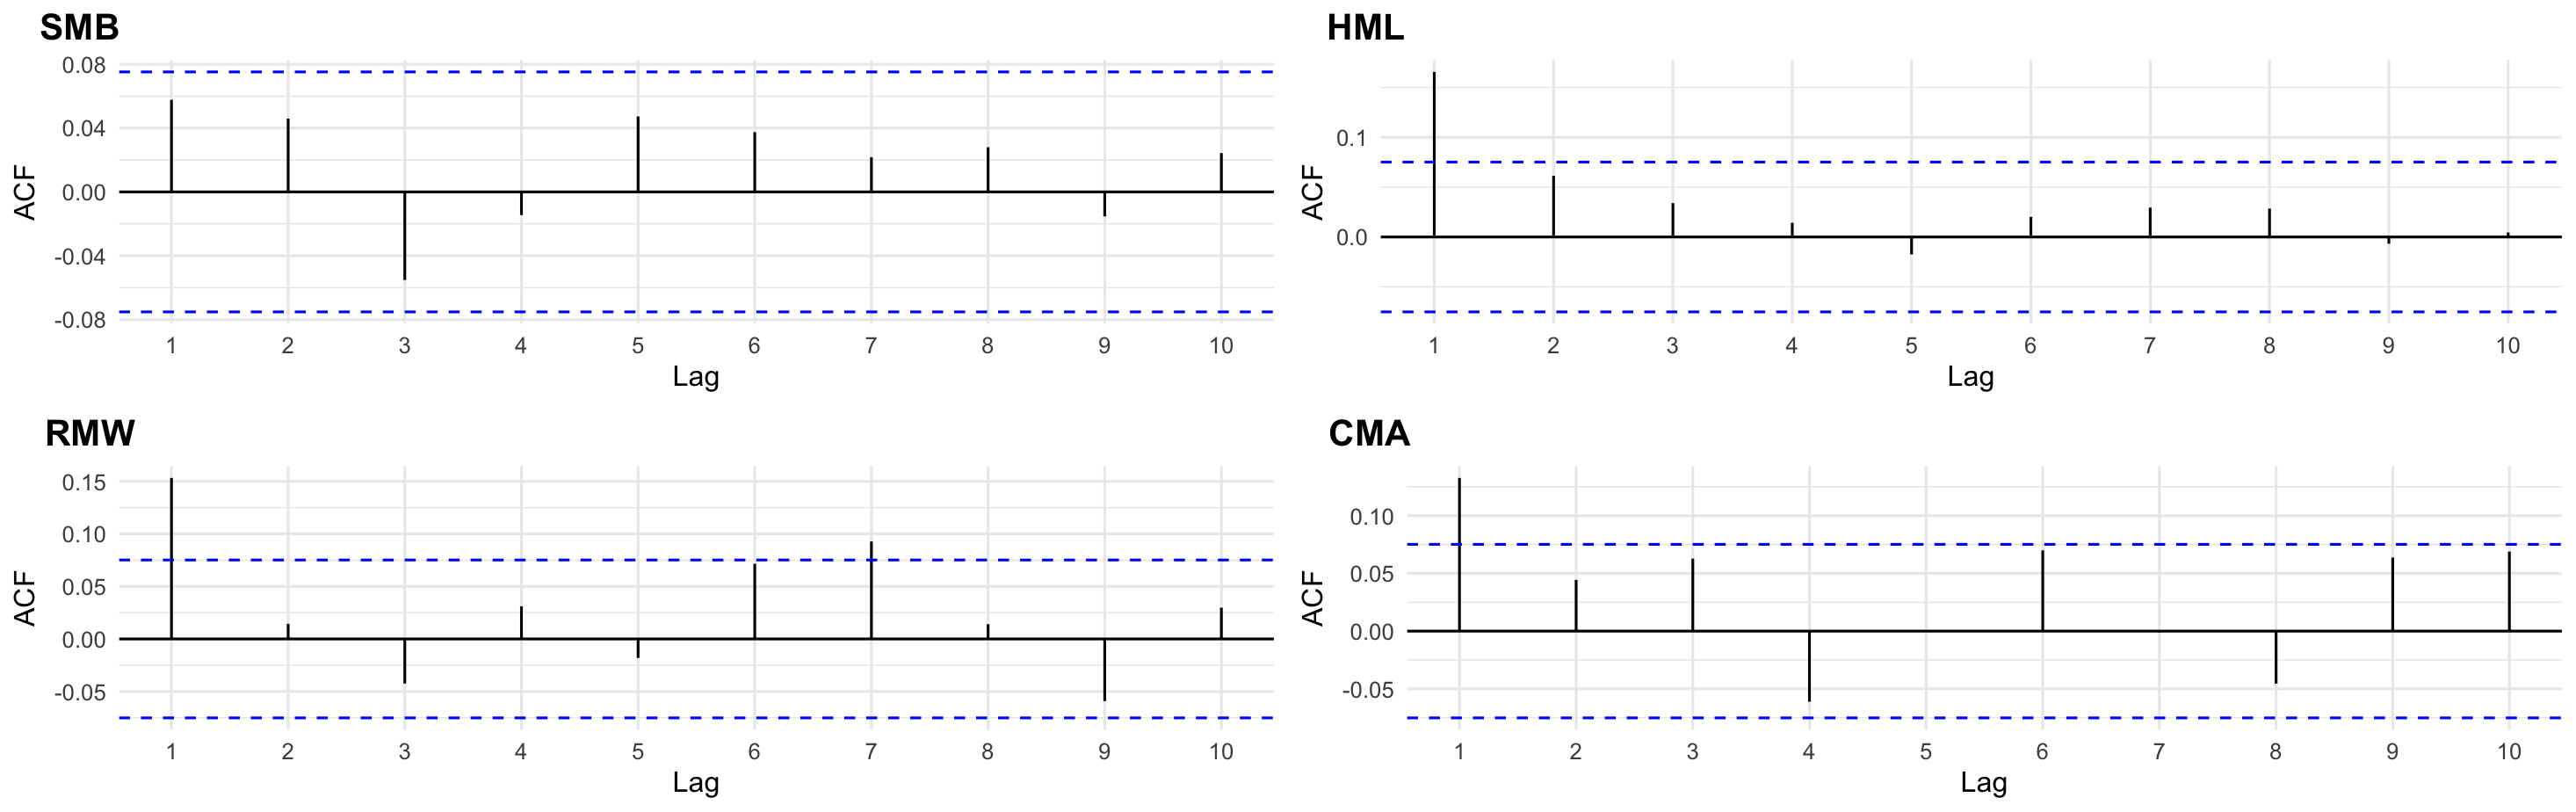
\includegraphics[width=\textwidth]{part_1/images/factor_autocorrelation.png}
\end{figure}

\subsubsection{Factor timing}
Given the abundance of evidence of the time-varying nature of factor premia, it is legitimate to wonder if it is possible to predict when factor will perform well or badly. The evidence on the effectiveness of timing is diverse. The majority of positive findings may be due to the bias towards positive results - but this is pure speculation.

There is no consensus on which predictors to use. A method for building reasonable timing strategies for long-only portfolios with sustainable transaction costs is laid out in Leippold and Rüegg (2020). The cross-section of characteristics is used for factor timing purposes in Kagkadis et al. (2021). In Vincenz and Zeissler (2021), it is found that macro variables are the best for this purpose. In ML-based factor investing, it is possible to resort to more granularity by combining firm-specific attributes to large-scale economic data.

\subsubsection{The green factors}

Demand for ethical financial products has risen lately. Not a new concept, but a lot more research has gone into if characteristics related to ESG criteria are priced or not (no consensus has been reached). Below are papers that suggest conflicting results:
\begin{itemize}[noitemsep]
    \item \textbf{Favorable}: ESG investing works (Kempf and Osthoff (2007), Cheema-Fox et al. (2020)), can work (Nagy, Kassam, and Lee (2016), Alessandrini and Jondeau (2020)), or can at least be rendered efficient (Branch and Cai (2012)). A large meta-study reports overwhelming favorable results (Friede, Busch, and Bassen (2015)), but of course, they could well stem from the publication bias towards positive results.
    \item \textbf{Unfavorable}: Ethical investing is not profitable according to Adler and Kritzman (2008) and Blitz and Swinkels (2020). An ESG factor should be long unethical firms and short ethical ones (Lioui (2018)).
    \item \textbf{Mixed}: ESG investing may be beneficial globally but not locally (Chakrabarti and Sen (2020)). Portfolios relying on ESG screening do not significantly outperform those with no screening but are subject to lower levels of volatility (Gibson et al. (2020), Gougler and Utz (2020)). As is often the case, the devil is in the details, and results depend on whether to use E, S or G (Bruder et al. (2019)).
\end{itemize}

ESG criteria can be directly integrated into a ML-model, as for instance done in France et al. (2020).

\subsection{Links with machine learning}
The task of linking alternative (\textit{e.g. sentiment data}) and traditional accounting data (\textit{e.g. accounting ratios}) is well suited for Machine Learning. Given a large set of predictor variables ($\mathbf{X}$), the goal is to predict a proxy for future performance $\mathbf{y}$ through a model of the firm discussed earlier
\begin{equation*}
    \mathbf{y} = f(\mathbf{X}) + \epsilon.
\end{equation*}

Earlier attempts have been made to predict and explain returns with firm attributes, but not with ML intents. However, these approaches share some links with ML tools. the general formulation; at time $T$, the agent/investor seeks to solve the following program
\begin{equation*}
    \max_{\mathbf{\theta}_{T}} \mathbb{E}_{T}[u(r_{p,T+1})] = \max_{\mathbf{\theta}_{T}} \mathbb{E}_{T}[u((\bar{\mathbf{w}}_T + \mathbf{x}_{T}\boldsymbol{\theta}_{T})' \mathbf{r}_{T+1})]
\end{equation*}
where $u$ is some utility function and $r_{p,T+1} = (\bar{\mathbf{w}}_T + \mathbf{x}_{T}\boldsymbol{\theta}_{T})' \mathbf{r}_{T+1}$ is the return of the portfolio, which is defined as a benchmark $\bar{\mathbf{w}}_T$ plus some deviations from this benchmark that are a linear function of features $\mathbf{x}_{T}\boldsymbol{\theta}$. This optimization may be subject to external constraints.

In practice $\boldsymbol{\theta }_{T}$ is estimated using past data (from $T-\tau$ to $T-1$). The agent seeks the solution of
\begin{equation}
    \max_{\boldsymbol{\theta}_{T}} \frac{1}{\tau} \sum_{t=T-\tau}^{T-1} u \left( \sum _{i=1}^{N_{T}} (\bar{w}_{i,t} + \boldsymbol{\theta}_{T}' \mathbf{x}_{i,t}) r_{i,t+1} \right)
\end{equation}
on a sample size of $\tau$ where $N_{T}$ is the number of assets in the market/universe. The above formulation can be viewed as a learning task in which the parameters are chosen such that the reward (average return) is maximized.

\subsubsection{Explicit connections with asset pricing models}
The first link between factor investing and asset pricing is (average) return prediction. The main canonical academic reference uses the following general equation
\begin{equation}
  r_{t+1,n} = g(\mathbf{x}_{t,n}) + \epsilon_{t+1} \label{eq:3.6}
\end{equation}

The discussion is in the differences between the discussion above and \eqref{eq:3}. 

The first difference is the non-linear function $g$: there is no reason to restrict the model to linear relationships. One early reference for nonlinearities in asset pricing kernels is Bansal and Viswanathan (1993).

The second difference between \eqref{eq:3} and \eqref{eq:3.6} is the shift in the time index. The interest is to be able to predict some information about the structure of the cross-section of assets. Explaining asset returns with synchronous factors is not useful because the realization of factor values is not known in advance. If we want to extract value from the model, there needs to be a time interval between the observation of the state space ($\mathbf{x}_{t,n}$) and the occurrence of the returns. 

With \eqref{eq:3.6}, ince $\hat{g}$ is estimated, the time-$t$ (measurable) value $g(\mathbf{x}_{t,n})$ will give a forecast for the (average) future returns. These predictions can then serve as signals in the crafting of portfolio weights. We can also replace returns with Sharpe ratios, amongst others.

Below are some ML-related tools that can be used to estimate asset pricing models.

\begin{thm}[Stochastic discount factor]
  The most mainstream problem in asset pricing is to characterize the stochastic discount factor (SDF) $M_{t}$, which satisfies $\mathbb{E}[M_{t+1}(r_{t+1,n} - r_{t+1,f})] = 0$ for any asset $n$. This equation is a natural playing field for the generalized method of moment: $M_{t}$ must be such that
  \begin{equation}
    \mathbb{E}[M_{t+1}R_{t+1,n}g(V_{t})] = 0 \label{eq:3.6}
  \end{equation}
  where the instrumental variables $V_{t}$ are $\mathcal{F}_t$-measurable (known at $t$) and the capital $R_{t+1,n}$ denotes the excess return of asset $n$.
\end{thm}

To simplify the problem define SDF as a portfolio of assets. Luyang Chen, Pelger, and Zhu (2020) use a generative adversarial network (GAN) to estimate the weights of the portfolios that are closest to satisfy \eqref{eq:3.6} under a strongly penalizing form. 

\begin{thm}[Linear combinations of factors]
  As done in \eqref{eq:5} we try to estimate returns as linear combinations of factors. We write in compact notation
  \[
    r_{t,n} = \alpha _{n} + \boldsymbol{\beta}'_{t,n} \mathbf{f}_{t} + \epsilon_{t,n}
  \]
  where loadings, $\boldsymbol{\beta}_{t,n}$ are time dependent. 
\end{thm}

To improve the model we want to introduce firm characteristics in the above equation. Traditionally, the characteristics are present in the definition of factors. The decomposition of the return is made according to the exposition of the firm's return to these factors constructed according to market size, accounting ratios, past performance, etc. Given the exposures, the performance of the stock is attributed to particular style profiles (\textit{e.g., small stock, or value stock, etc.}).

Habitually, the factors are heuristic portfolios constructed from simple rules like thresholding. For instance, firms below the 1/3 quantile in book-to-market are growth firms and those above the 2/3 quantile are the value firms. A value factor can then be defined by the long-short portfolio of these two sets, with uniform weights.

One of the advances enabled by machine learning is to automate the construction of the factors. It is for instance the approach of Feng, Polson, and Xu (2019). Instead of building the factors heuristically, the authors optimize the construction to maximize the fit in the cross-section of returns. The optimization is performed via a relatively deep feed-forward neural network and the feature space is lagged so that the relationship is predictive. Theoretically, the resulting factors help explain a substantially larger proportion of the in-sample variance in the returns. The prediction ability of the model depends on how well it generalizes out-of-sample.

A third method is proposed below.
\begin{thm}[Latent factors, dependent loadings]
  A third approach is that of Kelly, Pruitt, and Su (2019).Their idea is the opposite: factors are latent (unobserved) and it is the betas (loadings) that depend on the characteristics. This allows many degrees of freedom because in $r_{t,n} = \alpha _{n} + (\boldsymbol{\beta }_{t,n}(\mathbf{x}_{t-1,n}))'\mathbf{f}_{t} + \epsilon_{t,n}$ only the characteristics $\mathbf{x}_{t-1,n}$ are known and both the factors $\mathbf{f}_{t}$ and the functional forms $\boldsymbol{\beta}_{t,n}( \cdot )$ must be estimated. 
\end{thm}

The authors of this methods worked with a linear form, which is more tractable.

The fourth and final approach is below.
\begin{thm}[Combining neural networks]
  The first neural network takes characteristics $\mathbf{x}_{t-1}$ as inputs and generates factors loadings $\boldsymbol{\beta }_{t-1}(\mathbf{x}_{t-1})$. The second network transforms returns $\mathbf{r}_{t}$ into factor values $\mathbf{f}_{t}(\mathbf{r}_{t})$. The aggregate model can be written as
  \begin{equation}
    \mathbf{r}_{t} = \boldsymbol{\beta }_{t-1}(\mathbf{x}_{t-1})'\mathbf{f}_{t}(\mathbf{r}_{t}) + \boldsymbol{\epsilon}_{t} \label{eq:3.7}
  \end{equation}
  
  This is special since the output is also present in the input ($\mathbf{r}_{t}$).
\end{thm}

In machine learning, autoencoders (see Section 7.7.2) share the same property. Their aim, just like in principal component analysis, is to find a parsimonious nonlinear representation form for a dataset (in this case, returns). In \eqref{eq:3.7} the input is $\mathbf{r}_{t}$ and the output function is $\boldsymbol{\beta }_{t-1}(\mathbf{x}_{t-1})'\mathbf{f}_{t}(\mathbf{r}_{t})$. The aim is to minimize the difference between the two just as is any regression-like model

\begin{defn}[Autoencoders]
  Autoencoders are neural networks which have outputs as close as possible to the inputs with an objective of dimensional reduction. The innovation in Gu, Kelly, and Xiu (2020a) is that the pure autoencoder part is merged with a vanilla perceptron used to model the loadings. The structure of the neural network is summarized below
  \[
    \left.\begin{array}{rcl}\mathrm{returns~}(\mathbf{r}_{t})&\xrightarrow{NN_{1}}&\mathrm{factors~}(\mathbf{f}_{t}=NN_{1}(\mathbf{r}_{t}))\\\text{characteristics }(\mathbf{x}_{t-1})&\xrightarrow{NN_{2}}&\mathrm{loadings~}(\boldsymbol{\beta}_{t-1}=NN_{2}(\mathbf{x}_{t-1}))\end{array}\right\}\longrightarrow\mathrm{~returns~}(r_{t})
  \]
  A simple autoencoder would consist of only the first line of the model.
\end{defn}

\newpage

\section{Data preprocessing}

\subsection{Know your data}

First step: Make sure data is from a reliable provider.

Second step: Look at summary statistics. This includes first order moments (mean, median, etc.), but second order quantities (variance, covariance/correlation) are useful as they can hint at colinearities in data. 

Often models include so many predictors that it is unpractical to look at these metrics. Minimal verification is recommended. 
\begin{itemize}
    \item focus on a subset of predictors (e.g., the most important or ones commonly linked to factors);
    \item track outliers in the summary statistics (when maximum/median or median/minimum ratios are off).
\end{itemize}

Below is an example showing the distribution of correlations between features and the one month ahead return.
\begin{figure}[H]
    \centering
    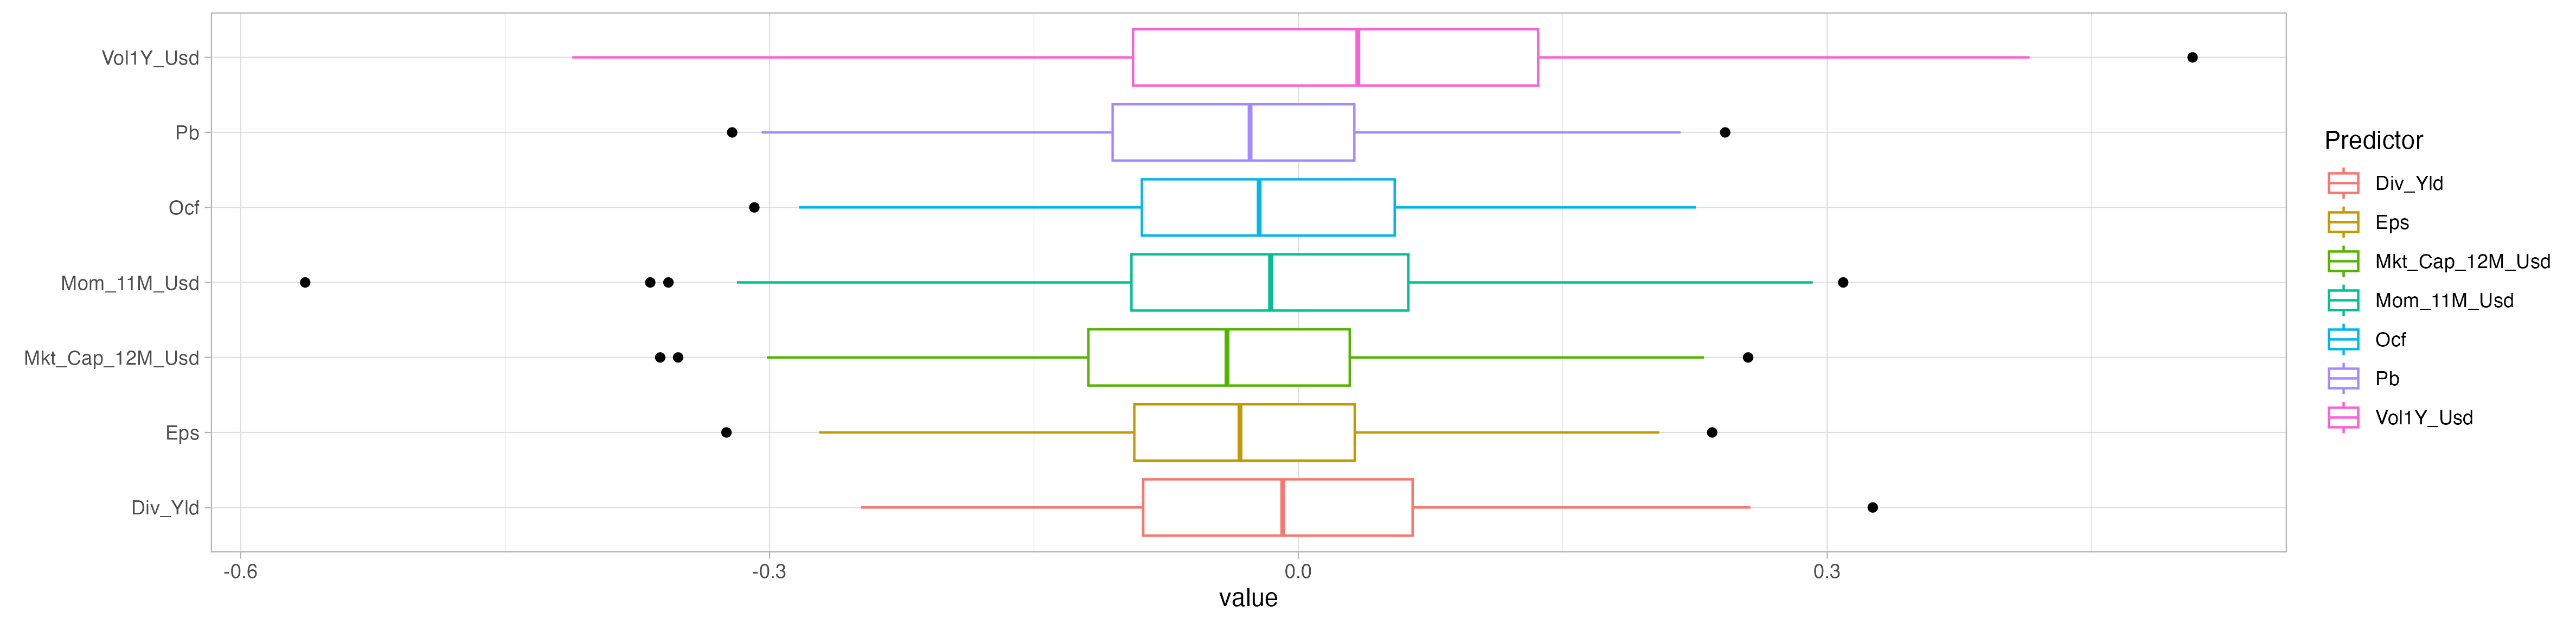
\includegraphics[width=\textwidth]{part_1/images/know_your_data_fig_1:boxplot.png}
\end{figure}

An important metric is the \textbf{smoothed conditional average} of the dependent variable on one feature. This can show the impact of a simple feature. 

Assume only one feature $X$ and we have the model $Y = f(X) + \text{error}$. The function $f$ which minimizes that average squared error $f(x) = \mathbb{E}[ (Y - f(X))^{2}]$ is the regression function:
\begin{equation}
    f(x) = \mathbb{E}[Y | X = x]
\end{equation}

Two examples of such a function are shown below, where the dependent variable is the one month ahead return. Note that both predictors have been uniformized (see later sections), so their values are uniformly distributed in the cross-section of assets for any given time period. The range of features is therefore $[0,1]$. Notice that the confidence interval is narrow when both (i) many data points are available, (ii) these datapoints are not too dispersed.
\begin{figure}[H]
    \centering
    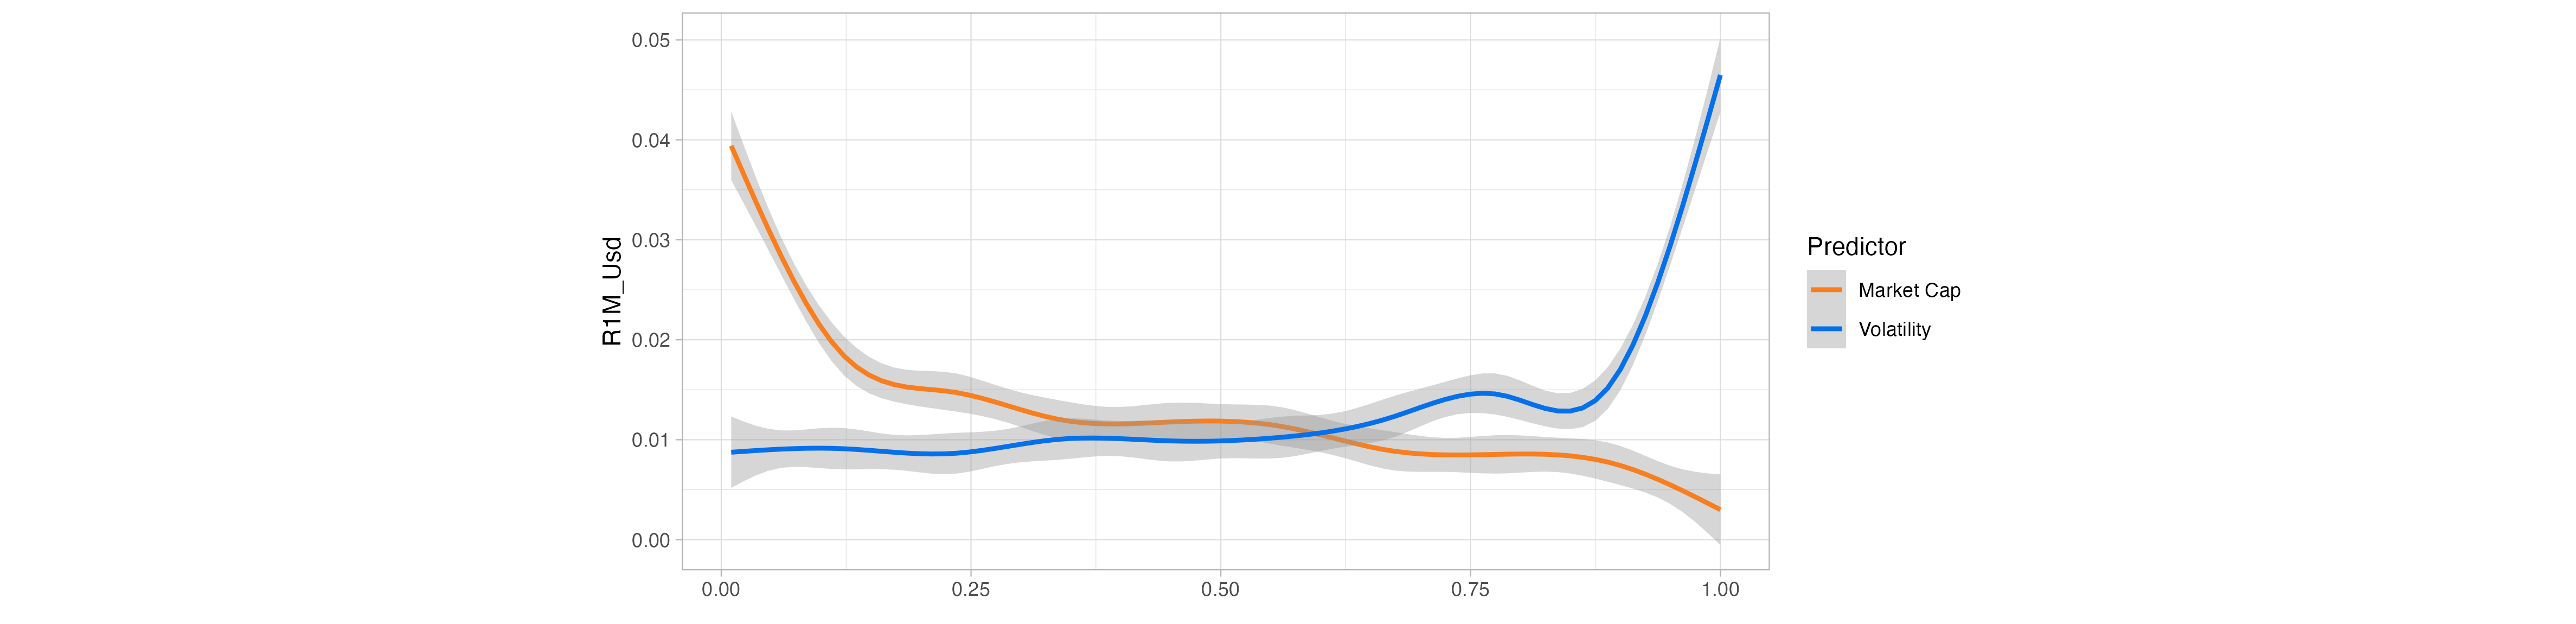
\includegraphics[width=\textwidth]{part_1/images/know_your_data_fig_2:sca.png}
\end{figure}
The two variables have a close to monotonic impact on future returns. Returns, on average, decrease with market capitalization (thereby corroborating the so-called size effect). The reverse pattern is less pronounced for volatility.


One important empirical property of features is autocorrelation (or absence thereof). A high level of \textbf{autocorrelation} for one predictor makes it plausible to use simple imputation techniques when some data points are missing. But autocorrelation is also important when moving towards prediction tasks. Autocorrelation has been calculated feature-by-feature and stock-by-stock in the plot below 
\begin{figure}[H]
    \centering
    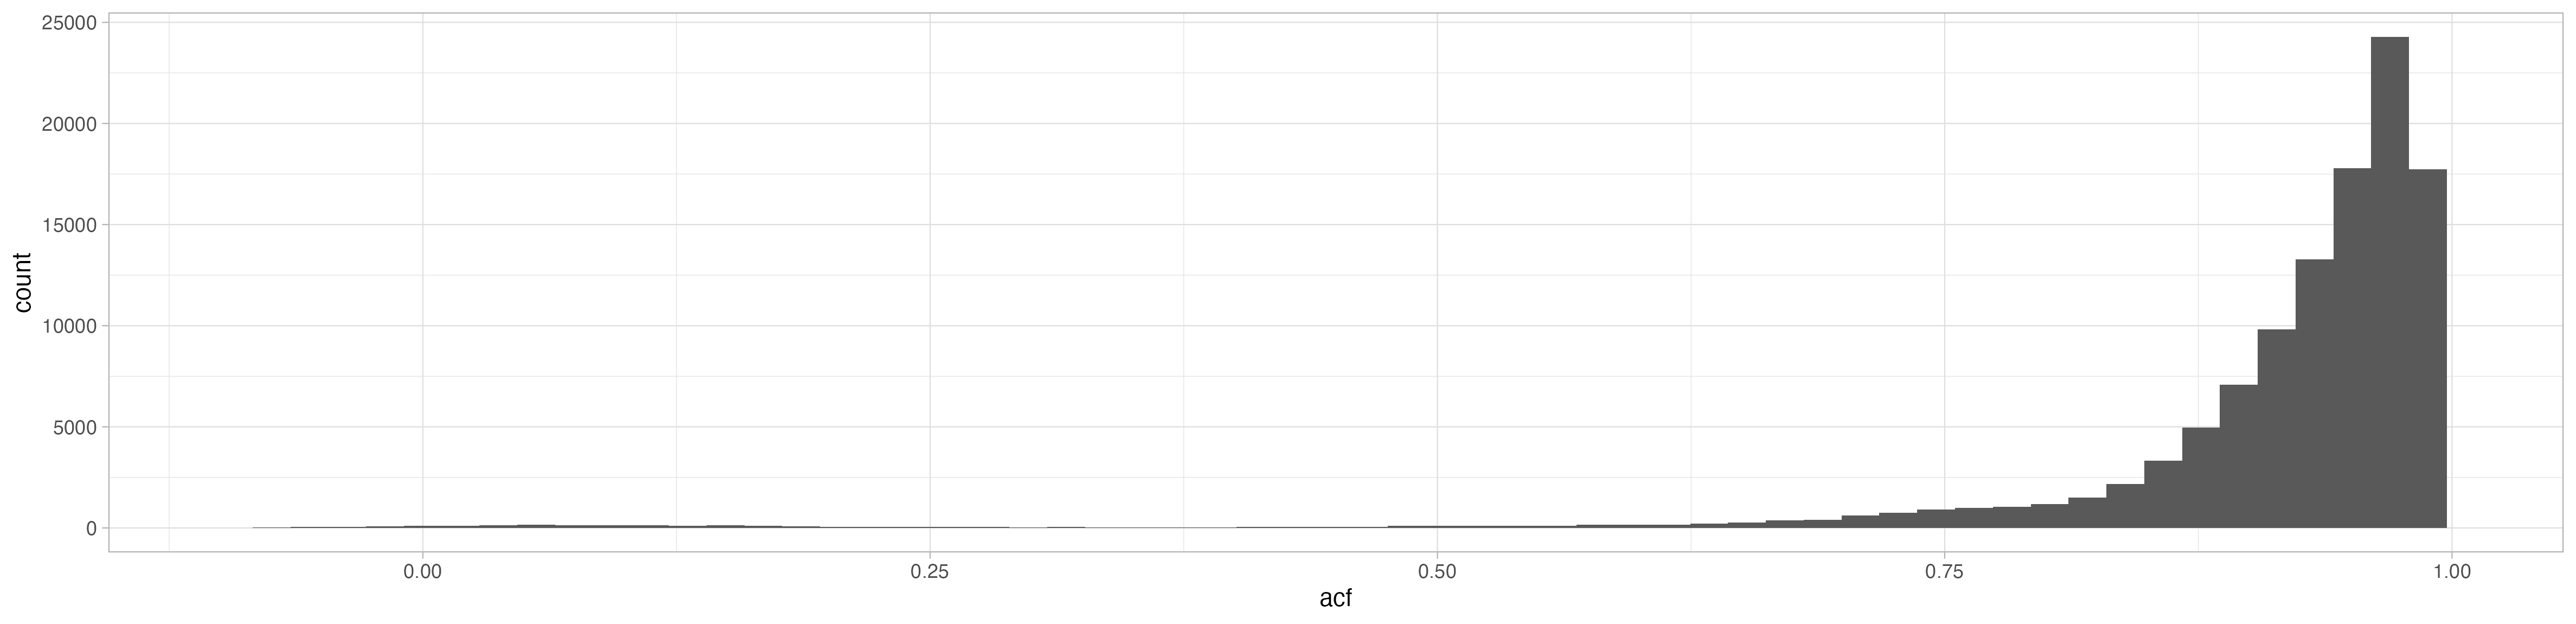
\includegraphics[width=0.6\textwidth]{part_1/images/know_your_data_fig_3:autocorr.png}
\end{figure}


We can see that predictors are highly correlated: most of them have autocorrelation around $0.8$.

\subsection{Missing data}
The methods for handling missing data are plentiful, but a simple heuristic approach is often sufficient. There are two ways of handling missing data: \textbf{removal} and \textbf{imputation}.Removal is agnostic but costly, especially if one whole instance is eliminated because of only one missing feature value. Imputation is often preferred but relies on some underlying and potentially erroneous assumption. 

Below is a simplified classification of imputation:
\begin{itemize}
    \item A basic imputation choice is the median (or mean) of the feature for the stock over the past available values. If there is a trend in the time series, this will nonetheless alter the trend. 
    \item In time series contexts with views towards backtesting, the most simple imputation comes from previous values: if $x_{t}$ is missing replace it with $x_{t-1}$. In some cases this is a very bad choice (see below).
    \item Medians and means can also be computed over the \textbf{cross-section} of assets. This roughly implies that the missing feature value will be relocated in the bulk of observed values. When many values are missing, this creates an atom in the distribution of the feature and alters the original distribution. One advantage is that this imputation is not forward-looking. 
    \item Other techniques rely on modelling assumptions for data generation. This will refer to non parametric approaches, which rely on random forests, Bayesian imputation, maximum likelihood approaches, interpolation or extrapolation adn nearest neighbor algorithms. Advanced techniques are much more demanding computationally.
\end{itemize}

A word of caution: 
\begin{itemize}
    \item Interpolation should be avoided at all costs. For example: Accounting values or ratios that are released every quarter must never be linearly interpolated for the simple reason that this is forward-looking. If numbers are disclosed in January and April, then interpolating February and March requires the knowledge of the April figure, which, in live trading will not be known. Resorting to past values is a better way to go.
    \item There are some feature types where imputation from past values should be avoided. E.g., returns should not be replicated. A better choice is to set the missing returns to zero (which is often close to the median or mean). An indicator that can be used in the decision is autocorrelation, which is the persistence of the feature through time. If a feature is highly autocorrelated then imputation from past values can make sense. If not, then avoid imputation. 
    \item There are cases that require more attention, and there are no out-of-the-box solutions. Consider a case of dividend yield released quarterly, in March, June, September, etc. We know the March value, but in June the data is missing. We do not know if there is a collection error where, or if the firm simply did not pay out any dividend in June. There are no perfect solutions, but for dividend data three options are: 1) Keep the previous value (use \codetext{na.locf()} is very good at this), 2) extrapolate from previous observations, 2) Set to zero (my be suboptimal due to dividend smoothing practices). For persistent time series the first two options are preferred.
\end{itemize}

Tests can be performed to evaluate the relative performance of each option. It is also important to remember these design choices. There are so many of them that they are easy to forget. Keeping track of them is obviously compulsory


\subsection{Outlier detection}
Incredibly sophisticated methods may require a lot of efforts for possibly limited gain. Simple heuristic methods, as long as they are documented in the process, may suffice. They often rely on hard thresholds
\begin{itemize}
    \item For one given feature (possibly filtered in time) any point outside the interval $[\mu - m \cdot \sigma; \mu + m \cdot \sigma]$ where often $m \in \{ 3,5,10 \} $ can be considered an outlier. 
    \item If the largest value is $m$ times above the second-to-largest, then it can be considered an outlier.
    \item For a give small threshold $q$, any value outside the $[q; 1-q]$ quantile range can be considered an outlier. 
\end{itemize}

The last idea is called \textbf{Winsorizing}, which is done by setting all values below $x^{(q)}$ to $x^{(q)}$ and values above $x^{(1-q)}$ to $x^{(1-q)}$. The winsorized variable is $\tilde{x}$
\[
    \tilde{x}_i = \begin{cases}
    x_{i} & \text{if } x_{i} \in [x^{(q)}, x^{(1-q)}] \\
    x^{(q)} & \text{if } x_{i} < x^{(q)} \\
    x^{(1-q)} & \text{if } x_{i} > x^{(1-q)} 
    \end{cases}
\]
where $q$ usually is $(0.5\%, 5\%)$ with 1\% and 2\% being the most commonly used. The winsorization stage \textbf{must} be performed on a feature-by-feature and a date-by-date basis.

We conclude this subsection by recalling that true outliers (i.e., extreme points that are not due to data extraction errors) are valuable because they are likely to carry important information.

\subsection{Feature engineering}
“Garbage in, garbage out”. It is paramount to prevent the ML engine of the allocation to be trained on ill-designed variable.

\subsubsection{Feature selection}
One heuristic choice is to chose the variables that are often mentioned in the literature (both academic and practical). Though of course, sticking to common characteristics may complicate the generation of alpha because all trading agents will take them into account. Choices can stem from empirical studies such as A. Y. Chen and Zimmermann (2021), or theoretical models like Ohlson (1995). 

Then, given a large set of predictors, it seems a sound idea to filter out unwanted or redundant exogenous variables. Heuristically, simple methods include:
\begin{itemize}
    \item computing the correlation matrix of all features and making sure that no (absolute) value is above a threshold (0.7 is a common value) so that redundant variables do not pollute the learning engine;
    \item carrying out a linear regression and removing the non significant variables (e.g., those with $p$-value above $0.05$);
    \item perform a clustering analysis over the set of features and retain only one feature within each cluster.
\end{itemize}

Both these methods are somewhat reductive and overlook nonlinear relationships. Another approach would be to fit a decision tree (or a random forest) and retain only the features that have a high variable importance. 

\subsubsection{Scaling the predictors}
The premise of the need to pre-process the data comes from the large variety of scales in financial data. While it is widely considered that monotonic transformations of the features have a marginal impact on prediction outcomes, Galili and Meilijson (2016) show that this is not always the case. 

If we write $x_{i}$, for the raw input and $\tilde{x}_i$ for the transformed data, common scaling practices include:
\begin{itemize}
    \item \textbf{standardization}: $\tilde{x}_{i} = (x_{i} - m_{x}) / \sigma _{x}$, where $m_{x}$ and $\sigma _{x}$ are the mean and standard deviation of $x_{i}$;
    \item \textbf{min-max} rescaling over $[0,1]$: $\tilde{x}_{i} = (x_{i} - \mathrm{min}(\mathbf{x})) / (\mathrm{max}(\mathbf{x}) - \mathrm{min}(\mathbf{x}))$; 
    \item \textbf{min-max} rescaling over $[-1,1]$: $\tilde{x}_i = 2 \cdot \frac{x_{i} - \mathrm{min}(\mathbf{x})}{\mathrm{max}(\mathbf{x}) - \mathrm{min}(\mathbf{x})} - 1$;
    \item \textbf{uniformization}: $\tilde{x}_i = F_{\mathbf{x}}(x_{i})$ , where $F_{\mathbf{x}}$ is the empirical c.d.f of $\mathbf{x}$. $\tilde{\mathbf{x}}$ is a vector uniformly distributed over $[0,1]$.
\end{itemize}

Sometimes, it is possible to apply a logarithmic transform of variables with both large values (market capitalization) and large outliers. The scaling can come after this transformation.

It is often advised to scale inputs so that they range in $[0,1]$ before sending them through the training of neural networks for instance.

In factor investing, the scaling of features must be \textbf{operated separately for each date and each feature}. This point is critical. It makes sure that for every rebalancing date, the predictors will have a similar shape and do carry information on the cross-section of stocks.

Scaling features across dates should be proscribed. Take for example the case of market capitalization. In the long run (market crashes notwithstanding), this feature increases through time. Thus, scaling across dates would lead to small values at the beginning of the sample and large values at the end of the sample. This would completely alter and dilute the cross-sectional content of the features.

\subsection{Labelling}

\subsubsection{Simple labels}
There are several ways to define labels when constructing portfolio policies. Of course, the finality is the portfolio weight, but it is rarely considered as the best choice for the label

Usual labels in factor investing are the following:
\begin{itemize}
    \item raw asset returns;
    \item future relative returns (versus some benchmark: market-wide index, or sector-based portfolio for instance). One simple choice is to take returns minus a cross-sectional mean or median;
    \item the probability of positive return (or of return above a specified threshold);
    \item the probability of outperforming a benchmark (computed over a given time frame);
    \item the binary version of the above: YES (outperforming) versus NO (underperforming);
    \item risk-adjusted versions of the above: Sharpe ratios, information ratios, MAR or CALMAR ratios.
\end{itemize}

When creating binary variables, it is often tempting to create a test that compares returns to zero. This is suboptimal because it is very time-dependent. It is a better idea to split the returns in two by comparing them to their time-$t$ median (or average). In this case, the indicator is relative and the two classes are much more balanced.



\subsubsection{Categorical labels}
In a typical ML analysis, when $y$ is a proxy for future performance, the ML engine will try to minimize some distance between the predicted value and the realized values. For mathematical convenience, the sum of squared error ($L^{2}$ norm) is used because it has the simplest derivative and makes gradient descent accessible and easy to compute.

Sometimes, it can be interesting not to focus on raw performance proxies, like returns or Sharpe ratios, but on discrete investment decisions, which can be derived from these proxies. A simple example (decision rule) is the following
\begin{equation}
    y_{t,i} = \begin{cases}
    -1 & \text{if } \hat{r}_{t,i} < r_{-} \\
    0 & \text{if } \hat{r}_{t,i} \in [r_{-}, r_{+}] \\
    1 & \text{if } \hat{r}_{t,i} > r_{+}
    \end{cases}
\end{equation}
where $\hat{r}_{t,i}$ is the performance proxy, $r_{\pm}$ are decision thresholds, and $-1$, $0$, and $1$ are the decisions (e.g., sell, hold, buy). It is often recommended that $r_{\pm}$ are chosen so the three categories are relatively balanced (have the same number of observations).

In this case, the final output can be considered as categorical or numerical because it belongs to an important subgroup of categorical variables: the ordered categorical (\textbf{ordinal}) variables. If $y$ is taken as a number, the usual regression tools apply.

When $y$ is treated as a non-ordered (\textbf{nominal}) categorical variable, then a new layer of processing is required because ML tools only work with numbers. Hence, the categories must be recoded into digits. The mapping that is most often used is called \textbf{one-hot encoding}. The vector of classes is split in a sparse matrix in which each column is dedicated to one class. The matrix is filled with zeros and ones. A one is allocated to the column corresponding to the class of the instance.

From the standpoint of allocation, handling categorical predictions is not necessarily easy. For long-short portfolios, plus or minus one signals can provide the sign of the position. For long-only portfolio, two possible solutions: (i) work with binary classes (in versus out of the portfolio) or (ii) adapt weights according to the prediction: zero weight for a -1 prediction, 0.5 weight for a 0 prediction and full weight for a +1 prediction. Weights are then of course normalized so as to comply with the budget constraint.

\subsubsection{Filtering the sample}
One of the main challenges in Machine Learning is to extract as much \textbf{signal} (patterns that will hold out-of-sample) as possible. Intuitively, it may seem reasonable to think that the more data we gather, the more signal we can extract. This is in fact false in all generality because more data also means more noise. Filtering the training samples can improve performance.

In Coqueret and Guida (2020), we investigate why smaller samples may lead to superior out-of-sample accuracy for a particular type of ML algorithm: decision trees (see Chapter 6). We focus on a particular kind of filter: we exclude the labels (e.g., returns) that are not extreme and retain the 20\% values that are the smallest and the 20\% that are the largest (the bulk of the distribution is removed). In doing so, we alter the structure of trees in two ways:
\begin{itemize}
    \item when the splitting points are altered, they are always closer to the center of the distribution of the splitting variable (i.e., the resulting clusters are more balanced and possibly more robust);
    \item the choice of splitting variables is (sometimes) pushed towards the features that have a monotonic impact on the label.
\end{itemize}

These two properties are desirable. The first reduces the risk of fitting to small groups of instances that may be spurious. The second gives more importance to features that appear globally more relevant in explaining the returns. However, the filtering must not be too intense (10\% filtering removes to much signal).

Several horizons come into play during the whole ML-driven allocation workflow: the \textbf{horizon of the label} (time period over which the outcome (label) is observed), the \textbf{estimation window} (chronological depth of the training samples / how much past data is used for training the model) and the \textbf{holding periods}. A paper analyzed different horizons for labels and holding (3,6,9,12). While there is no machine learning whatsoever in this contribution, it is possible that their conclusion that horizons matter may also hold for more sophisticated methods. This topic is in fact much discussed, as is shown by the continuing debate on the impact of horizons in momentum profitability.

This debate should also be considered when working with ML algorithms. In the present chapter, the horizon of the label is the important ingredient. Heuristically, there are four possible combinations if we consider only one feature for simplicity:
\begin{enumerate}
    \item oscillating label and feature;
    \item oscillating label, smooth feature (highly autocorrelated);
    \item smooth label, oscillating feature;
    \item smooth label and feature.
\end{enumerate}

Of all of these options, the last one is probably preferable because it is more robust. 


A pattern that holds between two slowly moving series is more likely to persist in time. Thus, since features are often highly autocorrelated, combining them with smooth labels is probably a good idea.

To illustrate how critical this point is, we will purposefully use 1-month returns in most of the examples of the book and show that the corresponding results are often disappointing. These returns are very weakly autocorrelated while 6-month or 12-month returns are much more persistent and are better choices for labels.

Theoretically, assume that returns are explained entirely by one feature $x_{t}$: $r_{t+1} = f(x_{t}) + \varepsilon_{t}$, where $x_{t}$ is highly autocorrelated and $\varepsilon_{t}$ is small. The compounded interest over multiple periods $(1 + r_{t+1}) (1 + r_{t+2}) - 1$ contains more meaningful signal than just $r_{t+1}$ alone. This suggests that incorporating memory effects into models (e.g., using longer time horizons or recurrent architectures) can improve predictions.

\subsection{Handling persistence}
Feature engineering and labelling have been separated into two different subsections, however i is best to consider them jointly. One important property of the dataset processed by the ML algorithm should be the consistency of persistence between features and labels. This means that autocorrelation patterns between label $y_{t,n}$ and the features $x_{t,n}^{(k)}$ should not be to distant.

Among other more technical options, there are two simple solutions when facing this issue: either introduce autocorrelation into the label, or remove it from the features. Again, the first option is not advised for statistical inference on linear models. Both are rather easy econometrically:
\begin{itemize}
    \item to increase the autocorrelation of the label compute performance over longer time ranges. For instance, when working with monthly data, considering annual or biennial returns will do the trick.
    \item To get rid of autocorrelation, the quickest way to do so is to resort to differences: $\Delta x_{t,n}^{(k)} = x_{t,n}^{(k)} - x_{t-1,n}^{(k)} $. An advantage of this procedure is that it makes sense, economically: variations in features my be better drivers of performance, compared to raw levels.
\end{itemize}

\subsection{Extensions}
\subsubsection{Transforming features}
The feature space can be augmented with simple operations. One of them is lagging (i.e., considering older values of features and assuming some memory effect for their impact on the label). This is useful mostly if the features are oscillating (adding a layer of memory on persistent feature can be redundant). New variables are defined by $\breve{x}_{t,n}^{(k)} = x_{t-1,n}^{(k)}$. 

In some cases (e.g., insufficient number of features), it is possible to consider ratios or products between features. Accounting ratios like price-to-book, book-to-market, debt-to-equity are examples of functions of raw features that make sense. The risk of overfitting increases, just like in a simple linear regression adding variables mechanically increases the $R^{2}$.

Another way to increase the feature space (mentioned above) is to consider differences. In this case, a new predictor is $\breve{x}_{t,n}^{(k)} = x_{t,n}^{(k)}  - x_{t-1,n}^{(k)}$.

\subsubsection{Macro-economic variables}
The data should never be separated from the context it comes from (its environment). In classical financial terms, this means that a particular model is likely to depend on the overarching situation which is often proxied by macro-economic indicators. One way to take this into account at the data level is simply to multiply the feature by an exogenous indicator $z_{t}$ and in this case, the new predictor is $\breve{x}_{t,n}^{(k)} = z_{t} \times x_{t,n}^{(k)}$.

Another route that integrates shifting economic environments is conditional engineering. Suppose that labels are coded via formula (4.2). The thresholds can be made dependent on some exogenous variable. It might be a good idea to adjust the thresholds based on the macro-economic state. One such example of dynamic thresholding is
\begin{equation}
    r_{t, \pm} = r_{\pm} \times e^{\pm \delta (\mathrm{VIX}_t - \bar{\mathrm{VIX}})}
\end{equation}
where $\mathrm{VIX}_{t}$ is the $t$ time value of the VIX index, and $\bar{\mathrm{VIX}}$ is some average og median value. The parameter $\delta $ tunes the magnitude of correction.

\chapter{Common supervised algorithms}

\section{Tree based methods}

Popular forecasting tools when working with tabular data.

\subsection{Simple trees}

\subsubsection{Principle}
Decision trees seek to partition datasets into homogeneous clusters. Given an exogenous variable $\boldsymbol{Y}$ and features $\boldsymbol{X}$ decision trees iteratively splits the sample into groups that are homogenous in $\boldsymbol{Y}$. The splits are made according to one variable within the set of features.

When $\boldsymbol{Y}$ consists of real numbers trees are regression trees, and when $\boldsymbol{Y}$ is categorical we talk about classification trees.

The purpose of the exercise is to find the characteristics that allow to split firms into the ones that will perform well versus those likely to fare more poorly.

Given a sample ($y_{i}$ and $\mathbf{x}_{i}$) of size $I$ a regression tree seeks splitting points that minimize total variation of $y_{i}$ inside the two child clusters (that do not need to have the same size).

First, it finds, for each feature $x_{i}^{(k)}$, the best splitting point. Second, it selects the feature that achieves the highest level of homogeneity in $\mathbf{Y}$.
Homogeneity in regression trees is closely linked to variance. since we want the $y_{i}$ inside each cluster to be similar we seek to minimize their variability (or dispersion) inside each cluster, and then sum the two figures. We cannot sum the variances because this would not take into account the relative sizes of clusters. Hence, we work with total variation (variance times the number of elements in each cluster).

The first step is to find the best split for each feature, that is solve $\mathrm{argmin}_{c^{(k)}} V^{(k)}_{I}(c^{(k)})$ with 
\begin{equation}
    V_{I}^{(k)} (c^{(k)}) = \sum_{x_{i}^{(k)} < c^{(k)}} (y_{i} - m_{I}^{k, -}(c^{(k)}))^{2} +  \sum_{x_{i}^{(k)} > c^{(k)}} (y_{i} - m_{I}^{k, +}(c^{(k)}))^{2}, 
\end{equation} 0 
where
\begin{align*}
    m_{I}^{k, -} &= \frac{1}{\# \{ i, x_{i}^{(k)} < c^{(k)} \} } \sum_{\{ x_{i}^{(k)} < c^{(k)} \} } y_{i} \\
    m_{I}^{k, +} &= \frac{1}{\# \{ i, x_{i}^{(k)} > c^{(k)} \} } \sum_{\{ x_{i}^{(k)} > c^{(k)} \} } y_{i}
\end{align*}
are the average values of $\boldsymbol{Y}$ , conditional on $\boldsymbol{X}^{(k)}$ being smaller or larger than $c$. For feature $k$, the optimal split $c^{k,\ast}$ is thus the one for which the total dispersion over the two subgroups is the smallest.

The optimal splits satisfy $c^{k, \ast} = \mathrm{argmin}_{c^{(k)}} V_{I}^{(k)} (c^{(k)})$. Of all the possible splitting variables, the tree will choose the one that minimizes the total dispersion not only over all splits, but also over all variables: $k^{\ast} = \mathrm{argmin}_{k} V_{I}^{(k)} (c^{k, \ast})$.

There are several criteria that can determine when to stop the splitting process. One simple criterion is to fix a maximum number of levels (the depth) for the tree. A usual condition is to impose a minimum gain that is expected for each split. If the reduction in dispersion after the split is only marginal and below a specified threshold, then the split is not executed.

When the tree is built (trained), a prediction for new instances is easy to make. Given its feature values, the instance ends up in one leaf of the tree. Each leaf has an average value for the label: this is the predicted outcome. Of course, this only works when the label is numerical. 

\subsubsection{Further details on classification}
Classification exercises are somewhat more complex than regression tasks. The most obvious difference is the measure of dispersion or heterogeneity. This loss function which must take into account the fact that the final output is not a simple number, but a vector. The output $\tilde{\mathbf{y}}_i$ has as many elements as there are categories in the label and each element is the probability that the instance belongs to the corresponding category.

Inside a tree, labels are aggregated at each cluster level. A typical output would look like (0.6,0.1,0.3): they are the proportions of each class represented within the cluster. In this case, the cluster has 60\% of buy, 10\% of hold and 30\% of sell.

The loss function must take into account this multidimensionality of the label. When building trees, since the aim is to favor homogeneity, the loss penalizes outputs that are not concentrated towards one class.

The algorithm is thus seeking purity: it searches a splitting criterion that will lead to clusters that are as pure as possible. If there are $J$ classes, we denote these proportions with $p_{J}$. For each leaf, the usual loss functions are:
\begin{itemize}
    \item the Gini impurity index: $1- \sum_{j=1}^{J} p_{j}^{2}$;
    \item the misclassification error: $1 - \max_{j} p_{j}$;
    \item entropy: $- \sum _{j=1}^{J} \log(p_{j})p_{j}$.
\end{itemize}

Once the tree is grown, new instances automatically belong to one final leaf. This leaf is associated to the proportions of classes it nests. Usually, to make a prediction, the class with highest proportion (or probability) is chosen when a new instance is associated with the leaf.

\subsubsection{Pruning criteria}
When building a tree, the splitting process can be pursued until the full tree is grown, that is, when:
\begin{itemize}
    \item all instances belong to separate leaves, and/or
    \item all leaves comprise instances that cannot be further segregated based on the current set of features.
\end{itemize}
At this stage, the splitting process cannot be pursued.

Obviously, fully grown trees often lead to almost perfect fits when the predictors are relevant, numerous and numerical. Nonetheless, the fine grained idiosyncrasies of the training sample are of little interest for out-of-sample predictions. For instance, being able to perfectly match the patterns of 2000 to 2006 will probably not be very interesting in the period from 2007 to 2009. The most reliable sections of the trees are those closest to the root because they embed large portions of the data: the average values in the early clusters are trustworthy because the are computed on a large number of observations. The first splits are those that matter the most because they determine the most general patterns. The deepest splits only deal with the peculiarities of the sample.

Thus, it is imperative to limit the size of the tree to avoid overfitting. There are several ways to prune the tree and all depend on some particular criteria. We list a few of them below:
\begin{itemize}
    \item Impose a minimum number of instances for each terminal node (leaf). This ensures that each final cluster is composed of a sufficient number of observations. Hence, the average value of the label will be reliable because it is calculated on a large amount of data.
    \item Similarly, it can be imposed that a cluster has a minimal size before even considering any further split. This criterion is of course related to the one above.
    \item Require a certain threshold of improvement in the fit. If a split does not sufficiently reduce the loss, then it can be deemed unnecessary. The user specifies a small number $\epsilon > 0$ and a split is only validated if the loss obtained post-split is smaller than $1-\epsilon $ times the loss before the split.
    \item Limit the depth of the tree. The depth is defined as the overal maximum number of splits between the root and any leaf of the tree.
\end{itemize}

\subsubsection{Code and interpretation}
See the jupyter notebook for the code. The plot below is a simple tree.

Notice that one peculiarity of trees is their possible heterogeneity in cluster sizes. Sometimes, a few clusters gather almost all of the observations while a few small groups embed some outliers. This is not a favorable property of trees, as small groups are more likely to be flukes and may fail to generalize out-of-sample.

This is why we imposed restrictions during the construction of the tree. The first one (minbucket = 3500 in the code) imposes that each cluster consists of at least 3500 instances. The second one (minsplit) further imposes that a cluster comprises at least 8000 observations in order to pursue the splitting process. These values logically depend on the size of the training sample. The cp = 0.0001 parameter in the code requires any split to reduce the loss below 0.9999 times its original value before the split. Finally, the maximum depth of three essentially means that there are at most three splits between the root of the tree and any terminal leaf.

Once the model has been trained (i.e., the tree is grown), a prediction for any instance is the average value of the label within the cluster where the instance should land.

As a verification of the first splits, we plot the smoothed average of future returns, conditionally on market capitalization, price-to-book ratio and trading volume.

The graph shows the relevance of clusters based on market capitalizations and price-to-book ratios. For low score values of these two features, the average return is high (close to +4\% on a monthly basis on the left of the curves). The pattern is more pronounced compared to volume for instance.

Finally, we assess the predictive quality of a single tree on the testing set.
\begin{lstlisting}
y_train = training_sample['R1M_Usd'].values
X_train = training_sample[features].values
y_test = testing_sample['R1M_Usd'].values
X_test = testing_sample[features].values


fit_tree2 = tree.DecisionTreeRegressor( # Definining the model
    min_samples_split = 4000, # Min nb of obs required to continue splitting
    max_depth = 5, # Maximum depth (i.e. tree levels)
    ccp_alpha=0.0001, # complexity parameters
    min_samples_leaf =1500 # Min nb of obs required in each terminal node (leaf)
        )
fit_tree2 = fit_tree2.fit(X_train, y_train) # Fitting the model

mse = np.mean((fit_tree2.predict(X_test) - y_test)**2)
print(f'MSE: {mse}')
hitratio = np.mean(fit_tree2.predict(X_test) * y_test > 0)
print(f'Hit Ratio: {hitratio}')
\end{lstlisting}
, which shows that  $\mathrm{MSE}: 0.036997$ and $\mathrm{Hit Ratio}: 0.546035$.

\subsection{Random forrest}
These models combine prediction models.

\subsubsection{Principle}
Most of the time, when having several modelling options at hand, it is not obvious upfront which individual model is the best, hence a combination seems a reasonable path towards the diversification of prediction errors (when they are not too correlated).

There are two ways to create multiple predictors from simple trees, and random forests combine both: 
\begin{itemize}
    \item first, the model can be trained on similar yet different datasets. One way to achieve this is via bootstrap.
    \item second, the data can be altered by curtailing the number of predictors. Alternative models are built based on different sets of features. The user chooses how many features to retain and then the algorithm selects these features randomly at each try.
\end{itemize}

Hence, it becomes simple to grow many different trees and the ensemble is simply a weighted combination of all trees. Usually, equal weights are used, which is an agnostic and robust choice.

Notably, Breiman (2001) shows that as the number of trees grows to infinity, the inaccuracy converges to some finite number which explains why random forests are not prone to overfitting.

\subsubsection{Code and results}

See jupyter notebook.

\subsection{Boosted trees: Adaboost}


In boosting, it is sought to iteratively improve the model whenever a new tree is added. Adaboost improves the learning process by progressively focusing on the instances that yield the largest errors.

\subsubsection{Methodology}

The general structure of the algorithm.
\begin{itemize}
    \item Set equal weights $w_{i} = I^{-1}$;
    \item For $m = 1,\dots, M$ do
    \begin{enumerate}
        \item Find a learner $l_{m}$ that minimizes the weighted loss $\sum _{i=1}^{I}w_{i}L(l_{m}(\mathbf{x}_{i}), \mathbf{y}_{i})$.
        \item Compute a learner weight
        \begin{equation}
            a_{m} = f_{a}(\mathbf{w}, l_{m}(\mathbf{x}), \mathbf{y});
        \end{equation}
        \item Update the instance weights
        \begin{equation}
            w_{i} \leftarrow w_{i} e^{ f_{w}(l_{m}(\mathbf{x}_{i}), \mathbf{y}_{i}) };
        \end{equation}
        \item Normalize the $w_{i}$ to sum to one;
    \end{enumerate}
    \item The output of the instance $x_{i}$ is a simple function of $\sum _{m=1}^{M}a_{m}l_{m}(\mathbf{x}_{i})$
    \begin{equation}
        \tilde{y}_{i} = f_{y} \left(\sum _{m=1}^{M}a_{m}l_{m}(\mathbf{x}_{i})\right)
    \end{equation}
\end{itemize}
This formulation work for many versions of Adaboost and the function $f_{a}$ and $f_{y}$ are specified below.

The first step is to find a tree ($l_{m}$) that minimizes a weighted loss. The loss function depends on the application. The second and third step define the way the algorithm adapts sequentially. A more sophisticated approach compared to uniform weights, is to assign a tailored weight to each learner. A property of $f_{a}$  should be that a learner that yields a smaller error should have a larger weight because it is more accurate. 

The third step s is to change the weights of observations. Since the models seeks to improve the learning process, $f_{w}$ is constructed to give more weight on observations for which the current model does not do a good job. The next learner (tree) will focus more on these pathological cases.

The final step is a scaling procedure. Below are two different weighting functions.

\begin{table}[H]
    \centering
    \resizebox{\textwidth}{!}{
        \begin{tabular}{ccc}
            \toprule
              & Bin. classif & Regression \\ \midrule
            Individual error & $\epsilon _{i} = \mathbf{1}_{\{ y_{i} \neq  l_{m}(\mathbf{x}_{i}) \} }$ & $\epsilon_i=\frac{	y_i- l_m(\textbf{x}_i)	}{\underset{i}{\max}y_i- l_m(\textbf{x}_i)}$ \\ 
            Weight of learner via §$f_{a}$ & $f_{a} = \log \left(\frac{1-\epsilon }{\epsilon } \right)$ with $\epsilon  = I^{-1} \sum _{i=1}^{I} w_{i} \epsilon _{i}$ & $f_{a} = \log \left(\frac{1-\epsilon }{\epsilon } \right)$ with $\epsilon  = I^{-1} \sum _{i=1}^{I} w_{i} \epsilon _{i}$ \\
            Weight of instances via $f_{w}(i)$ & $f_{w} = f_{a}\epsilon _{i}$ & $f_{w} = f_{a}\epsilon _{i}$ \\
            Output function via $f_{y}$ & $f_{y}(x) = \mathrm{sign}(x)$ & weighted median of predictions \\
            \bottomrule
        \end{tabular}
    }
\end{table}


\end{document}  